%! Author = murfe
%! Date = 09.09.2026

\chapter{Umsetzung}
\label{ch:umsetzung}
Dieses Kapitel befasst sich mit dem Entwurf und der technischen Umsetzung des in \cref{ch:anforderungen} definierten Systems.
Der Aufbau des Kapitels gliedert sich dabei in zwei Abschnitte:
Im ersten Teil wird die Architektur des Systems entwickelt und die fundamentalen Systementscheidungen begründet.
Aufbauend auf diesem theoretischen Fundament dokumentiert der zweite Teil die konkrete Implementierung des Prototyps auf
Basis des Java- und Spring-Ökosystems.

\section{Architektur und Design}
\label{sec:architektur}
In diesem Kapitel wird die Architektur des entwickelten Job-Processing-Systems zur Erfüllung von \ref{item:tz2} beschrieben.
Das primäre Ziel besteht darin, die in \cref{ch:anforderungen} erhobenen Anforderungen und Zusicherungen durch geeignete
Entwurfsentscheidungen und den gezielten Einsatz von Entwurfsmustern zu erfüllen.
Zur strukturierten Darstellung der einzelnen Systemkomponenten gliedert sich das Kapitel in folgende Teilaspekte:
\cref{subsec:architekturentwurf} führt zunächst in die abstrakte Gesamtsystemarchitektur ein, begründet die Wahl einer relationalen
PostgreSQL-Datenbank als zentralen Job-Store und stellt die Interaktion zwischen den einzelnen Komponenten dar.
Darauf aufbauend beschreibt \cref{subsec:zustandsmodell} das Zustandsmodell, welches unter anderem als Grundlage für die
Koordination der Jobs und die Recovery dient.
Das zugehörige Datenbankschema wird in \cref{subsec:datenbankentwurf} vorgestellt, während \cref{subsec:joberstellung}
die Mechanismen zur idempotenten Annahme neuer Jobs über \gls{rest} erläutert.
In \cref{subsec:transaktionsmodell} wird das Transaktions- und Sperrmodell betrachtet, das eine exklusive
Verarbeitung bei gleichzeitig kurzen Datenbanktransaktionen ermöglicht.
Anschließend widmen sich \cref{subsec:retryStrategie} und \cref{subsec:recoveryarchitektur} der Umsetzung von Retries und Recovery.
\Cref{subsec:idempotenteErgebnisgenerierung} schließt den Entwurf ab, indem die Nutzung des \textit{Fencing}-Prinzips zur Vermeidung
von Mehrfachverarbeitungen im Fehlerfall dargelegt wird.

\subsection{Architekturentwurf}
\label{subsec:architekturentwurf}
In \cref{subsec:backgroundJobs} wurde bereits dargelegt, dass das Queue-Based Load Leveling Pattern eine mögliche und etablierte
Option ist, ausstehende Jobs innerhalb eines Backend-Job-Processing-Systems zwischenzuspeichern.
Eine verbreitete Variante, dieses Pattern für Nachrichten, oder wie im Fall dieser Arbeit für Jobs, umzusetzen,
ist die Implementierung mithilfe dedizierter Message Broker \parencite[Kap.~11 Abschnitt \glqq Message brokers\grqq]{kleppmann_designing_2017}.
Wie bereits in \cref{sec:problemstellung} motiviert, wird im Rahmen dieser Arbeit hingegen untersucht, ob sich die definierten
Zusicherungen auch ohne eine solche zusätzliche Broker-Infrastruktur, allein mittels einer Datenbank, umsetzen lassen.

Aus den verschiedenen möglichen Datenbanksystemen fällt die Wahl auf eine relationale Datenbank.
Ausschlaggebend hierfür ist, dass mehrere der in \cref{sec:zusicherungen} hergeleiteten Zusicherungen starke Konsistenzgarantien voraussetzen.
Die exklusive Beanspruchung eines Jobs durch genau einen Worker (\ref{zus:exklusive_rechte}) erfordert eine Sperrmechanik auf Zeilenebene,
während atomare Persistierung von Statusänderung und fachlichem Ergebnis (\ref{zus:atomare_wirkung}) eine Transaktion voraussetzt,
die mehrere Schreiboperationen unteilbar zusammenfasst.
Viele der etablierten relationalen Datenbanksysteme stellen diese Eigenschaften in Form der \gls{acid}-Garantien als Bestandteil
ihres Transaktionsmodells bereit, wodurch sie sich für die vorliegende Problemstellung unmittelbar anbieten.

Als konkretes relationales Datenbanksystem wird PostgreSQL eingesetzt.
Ausschlaggebend hierfür ist die Kombination aus freier Verfügbarkeit, weiter Verbreitung sowie einer ausgereiften und
gut dokumentierten Unterstützung genau der Funktionalitäten, die für die vorliegende Architektur benötigt werden: exklusive
Zeilensperren mittels \texttt{SELECT ... FOR UPDATE} sowie deren nicht blockierende Variante mit \texttt{SKIP LOCKED},
die mit einem pull-basierten Claiming mehreren Workern eine effiziente, gegenseitig nicht blockierende Datenauswahl ermöglicht.
Durch den Einsatz dieser Mechanismen lässt sich bereits ein Teil der in \cref{sec:zusicherungen} erhobenen Anforderungen unmittelbar
durch inhärente Datenbankfunktionen realisieren.
Die Wahl von PostgreSQL stellt dabei einen bewussten Architektur-Trade-off dar.
Im Gegensatz zu In-Memory-Lösungen wie Redis entstehen durch das Schreiben auf den
Sekundärspeicher deutlich höhere Latenzen und Zugriffszeiten als bei reinen Hauptspeicherzugriffen.
Demgegenüber garantiert PostgreSQL die Dauerhaftigkeit eines Datensatzes, der in einer durch einen erfolgreichen Commit
abgeschlossenen Transaktion persistiert wurde.
Dieser Kompromiss wird bewusst eingegangen, weil Dauerhaftigkeit im Rahmen von \ref{zus:verarbeitungsgarantie} eine
zentrale Anforderung des entwickelten Systems ist.
Eine rein speicherresidente Alternative müsste entweder Datenverlust bei einem Absturz in Kauf nehmen oder ihrerseits einen
eigenen, synchronen Persistenzmechanismus implementieren, wodurch derselbe Latenz- und Durchsatzkompromiss nur potenziell
an eine andere Stelle verschoben wird.
Die grundsätzliche Eignung des gewählten Ansatzes ist jedoch nicht auf PostgreSQL beschränkt, sondern auf die Klasse
relationaler Datenbanksysteme mit entsprechender Unterstützung für nicht blockierende Sperrmechanismen und \gls{acid}-Garantien übertragbar.

Die Datenbank dient im System nicht nur als persistenter Datenspeicher, sondern fungiert gleichzeitig als Koordinations-
und Synchronisationsmechanismus für konkurrierende Worker.
Die Kombination aus Job-Store und fachlichen Daten in derselben relationalen Datenbank hat den Vorteil, dass
atomare Zustandsübergänge und eine konsistente Wiederherstellung des Systemzustands nach Fehlern ermöglicht werden,
ohne dass dabei die in \cref{sec:problemstellung} beschriebene Konsistenzproblematik zwischen getrennten Systemen auftritt.
Gerade für kleine bis mittelgroße Systeme, in deren Anwendungskontext kein Jobverlust auftreten darf, stellt der gewählte
Ansatz damit eine geeignete Architektur dar, da auf eine aufwändige Clusterstruktur mit Replikation der Daten zur Absicherung von
Jobverlusten verzichtet werden kann \parencite[Kap.~8 Abschnitt \glqq How Brokers Work (In A Nutshell)\grqq]{newman_building_2026}.

Die resultierende Gesamtarchitektur ist in \cref{fig:componentDiagram} dargestellt.
Eine detaillierte Bausteinsicht findet sich im Anhang in \cref{fig:detailBausteinsicht}.
Der Client bildet den Einstiegspunkt des Systems und erzeugt neue Jobs, die entsprechend \ref{req:rest} über eine
\gls{rest}-Schnittstelle an das Backend übertragen werden.
Im Rahmen des entwickelten Prototyps erfolgt dies direkt über einen Service, der die Kommunikation mit dem Backend-\gls{api} kapselt.
In der Praxis kann diese Komponente ebenso durch eine grafische Benutzeroberfläche oder eine externe Anwendung angesprochen werden.

\begin{figure}[h]
    \centering
    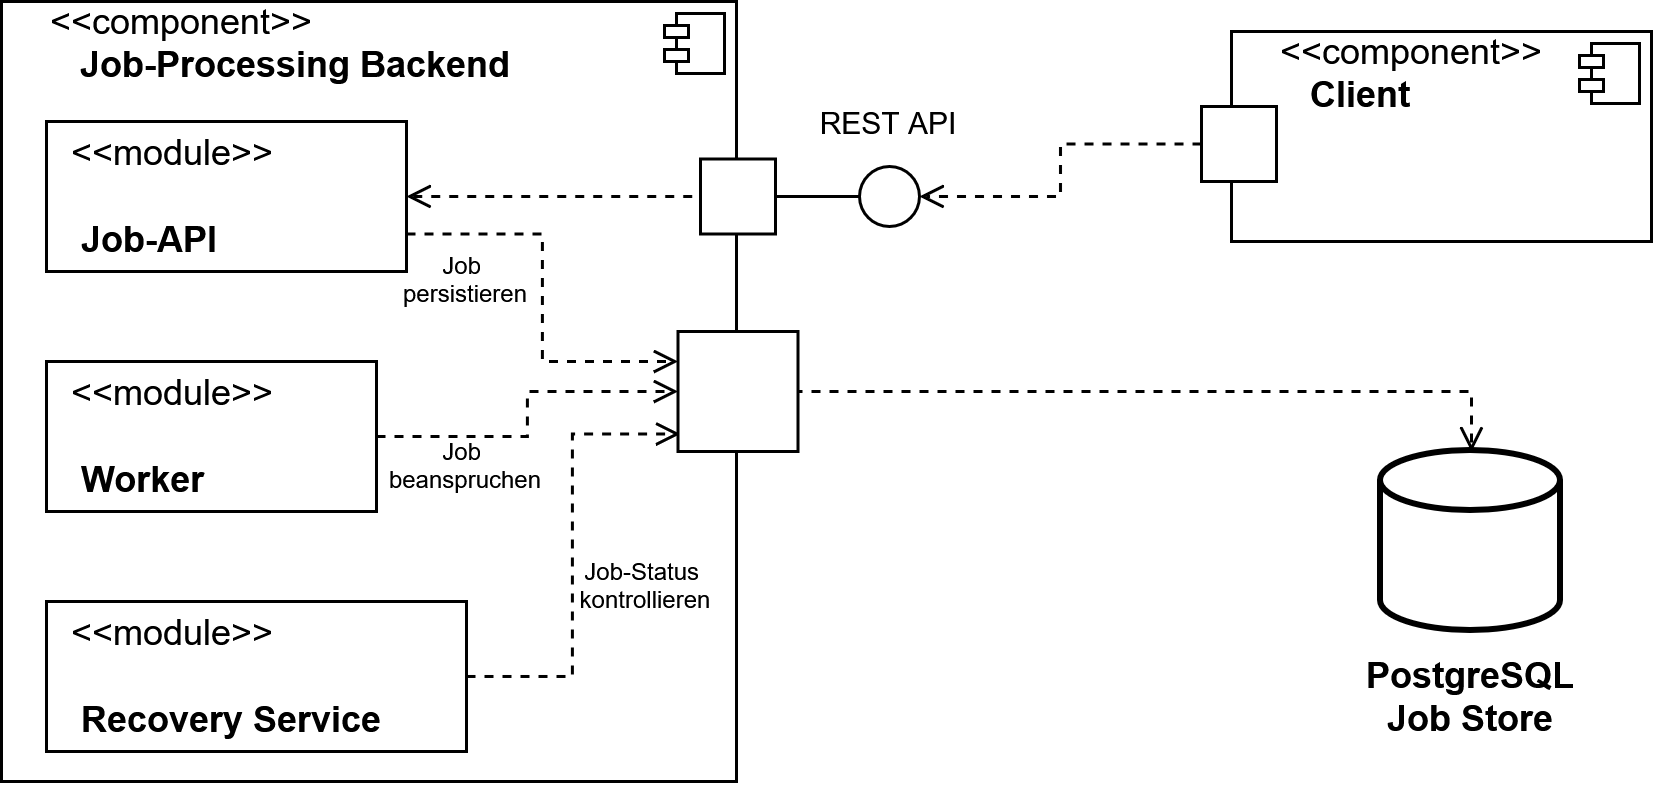
\includegraphics[width=0.8\textwidth]{images/componentDiagram}
    \caption[Bausteinsicht der Architektur des entwickelten Systems]{Bausteinsicht der Architektur des entwickelten
    Background-Job-Processing-Systems mit \gls{rest}-Schnittstelle, Job-Store sowie der Worker-Komponente und dem Recovery-Service.}
    \label{fig:componentDiagram}
\end{figure}

Die \gls{rest}-\gls{api} dient somit als Schnittstelle zur Joberstellung.
Sie validiert eingehende Anfragen (\ref{zus:atomare_persistenz}) und delegiert sie an die Servicelogik,
die für die Persistierung neuer Jobs sowie die Verwaltung ihrer Zustände verantwortlich ist.
Alle Jobs werden anschließend im zentralen Job-Store gespeichert (\ref{req:persistenz}), der neben den eigentlichen Jobdaten auch den aktuellen
Bearbeitungszustand sowie gegebenenfalls erzeugte Ergebnisse enthält.

Die eigentliche Verarbeitung erfolgt durch mehrere parallel arbeitende Worker (\ref{req:worker}).
Jeder Worker beansprucht einen Job exklusiv aus dem Job-Store, verarbeitet dessen Nutzdaten und speichert das erzeugte Ergebnis
anschließend wieder in der Datenbank.
Da sämtliche Worker auf denselben Job-Store zugreifen, kann die Verarbeitung durch Synchronisation auf Datenbankebene horizontal
skaliert werden, ohne dass eine direkte Kommunikation zwischen den einzelnen Workern erforderlich ist.

Ergänzt wird die Architektur durch einen Recovery-Service, der den Job-Store periodisch auf verwaiste Jobs überprüft.
Kann ein Worker einen bereits beanspruchten Job aufgrund eines Fehlers oder Absturzes nicht erfolgreich abschließen,
erkennt der Recovery-Service anhand des abgelaufenen Leases, dass die Bearbeitung nicht abgeschlossen wurde.
Der Status des betroffenen Jobs wird, sofern der Recovery-Service eine erneute Bearbeitung für sinnvoll erachtet,
zurückgesetzt und steht damit einem beliebigen Worker erneut zur Bearbeitung zur Verfügung.
Auf diese Weise wird verhindert, dass Jobs dauerhaft im Zustand \textit{Running} verbleiben (\ref{zus:terminierung})
oder infolge eines Worker-Ausfalls verloren gehen (\ref{zus:verarbeitungsgarantie}).

\subsection{Zustandsmodell}
\label{subsec:zustandsmodell}
Zur Realisierung der in \cref{ch:anforderungen} definierten Zusicherungen \ref{zus:exklusive_rechte}, \ref{zus:endzustaende},
\ref{zus:verarbeitungsgarantie}, \ref{zus:idempotenz} und \ref{zus:terminierung} wird jeder Job durch ein explizites Zustandsmodell beschrieben.
Der aktuelle Zustand eines Jobs wird dabei als Attribut des jeweiligen Datensatzes in der Datenbank gespeichert (vgl. \cref{subsec:datenbankentwurf})
und beschreibt den Fortschritt der Verarbeitung.
Das Zustandsmodell bildet die Grundlage für sämtliche Entscheidungen bezüglich der Bearbeitung, Wiederherstellung und Beendigung eines Jobs.
Ein wesentlicher Vorteil dieses Ansatzes besteht darin, dass Datenbankzeilen nicht über den gesamten Verarbeitungszeitraum
exklusiv gesperrt werden müssen.
Sperren sind lediglich während kurzer atomarer Zustandsübergänge erforderlich, während die eigentliche Verarbeitung
außerhalb einer Datenbanktransaktion erfolgt.
Dadurch werden Datenbankressourcen geschont, was sich positiv auf die Skalierbarkeit des Systems auswirkt.
Die in diesem System definierten Zustände sowie die zulässigen Zustandsübergänge sind in \cref{fig:statusmodell} dargestellt.

\begin{figure}[h]
    \centering
    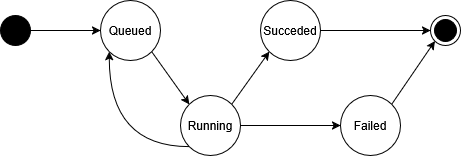
\includegraphics[width=0.8\textwidth]{images/statusmodell}
    \caption[Zustandsmodell eines Jobs]{Zustandsmodell eines Jobs mit den Zuständen \textit{Queued}, \textit{Running},
        \textit{Succeeded} und \textit{Failed} sowie den möglichen Zustandsübergängen während Annahme, Verarbeitung und Recovery.}
    \label{fig:statusmodell}
\end{figure}

Nachdem ein Job über die \gls{rest}-Schnittstelle im Backend eingegangen ist, wird dieser in den Zustand \textit{Queued}
versetzt und persistent gespeichert.
In diesem Zustand wartet der Job auf seine Bearbeitung und kann von einem Worker beansprucht werden.
Beansprucht ein Worker den Job erfolgreich, erfolgt der Zustandsübergang nach \textit{Running}.
Dadurch wird sichergestellt, dass der Job während seiner Verarbeitung keinem weiteren Worker zur Verfügung steht.
Zur Verarbeitung existieren drei mögliche Folgezustände.
Kann der Worker den Job erfolgreich bearbeiten und das erzeugte Ergebnis in der Datenbank speichern, wird der
Job in den Endzustand \textit{Succeeded} überführt.
Beendet der Worker seine Arbeit nicht innerhalb der vorgesehenen Lease-Dauer, beispielsweise weil ein Fehler auftritt,
übernimmt der Recovery-Service die weitere Behandlung des Jobs.
Ist gemäß der definierten Recovery-Strategie ein erneuter Ausführungsversuch zulässig, wird der Job zurück in den Zustand
\textit{Queued} versetzt und kann erneut von einem beliebigen Worker übernommen werden.
Wurde dagegen die maximale Anzahl zulässiger Wiederholungsversuche erreicht oder liegt ein als permanent eingestufter Fehler vor,
wird der Job in den Endzustand \textit{Failed} überführt.
Jobs in diesem Zustand werden vom System nicht weiter verarbeitet und erfordern ein manuelles Eingreifen.

\subsection{Entwurf der Datenbank}
\label{subsec:datenbankentwurf}
Die relationale Datenbank bildet den zentralen Job-Store des entwickelten Systems.
Durch die Nutzung einer relationalen Datenbank mit \gls{acid}, wird automatisch die in \ref{zus:atomare_persistenz}
und \ref{zus:verarbeitungsgarantie} geforderte Dauerhaftigkeit angenommener Jobs garantiert.
Sie übernimmt sowohl die Persistierung eingehender Jobs als auch die Verwaltung ihres aktuellen Bearbeitungszustands
und gegebenenfalls erzeugter Verarbeitungsergebnisse.
Das resultierende Datenbankschema ist in \cref{fig:dbSchema} dargestellt.

\begin{figure}[h]
    \centering
    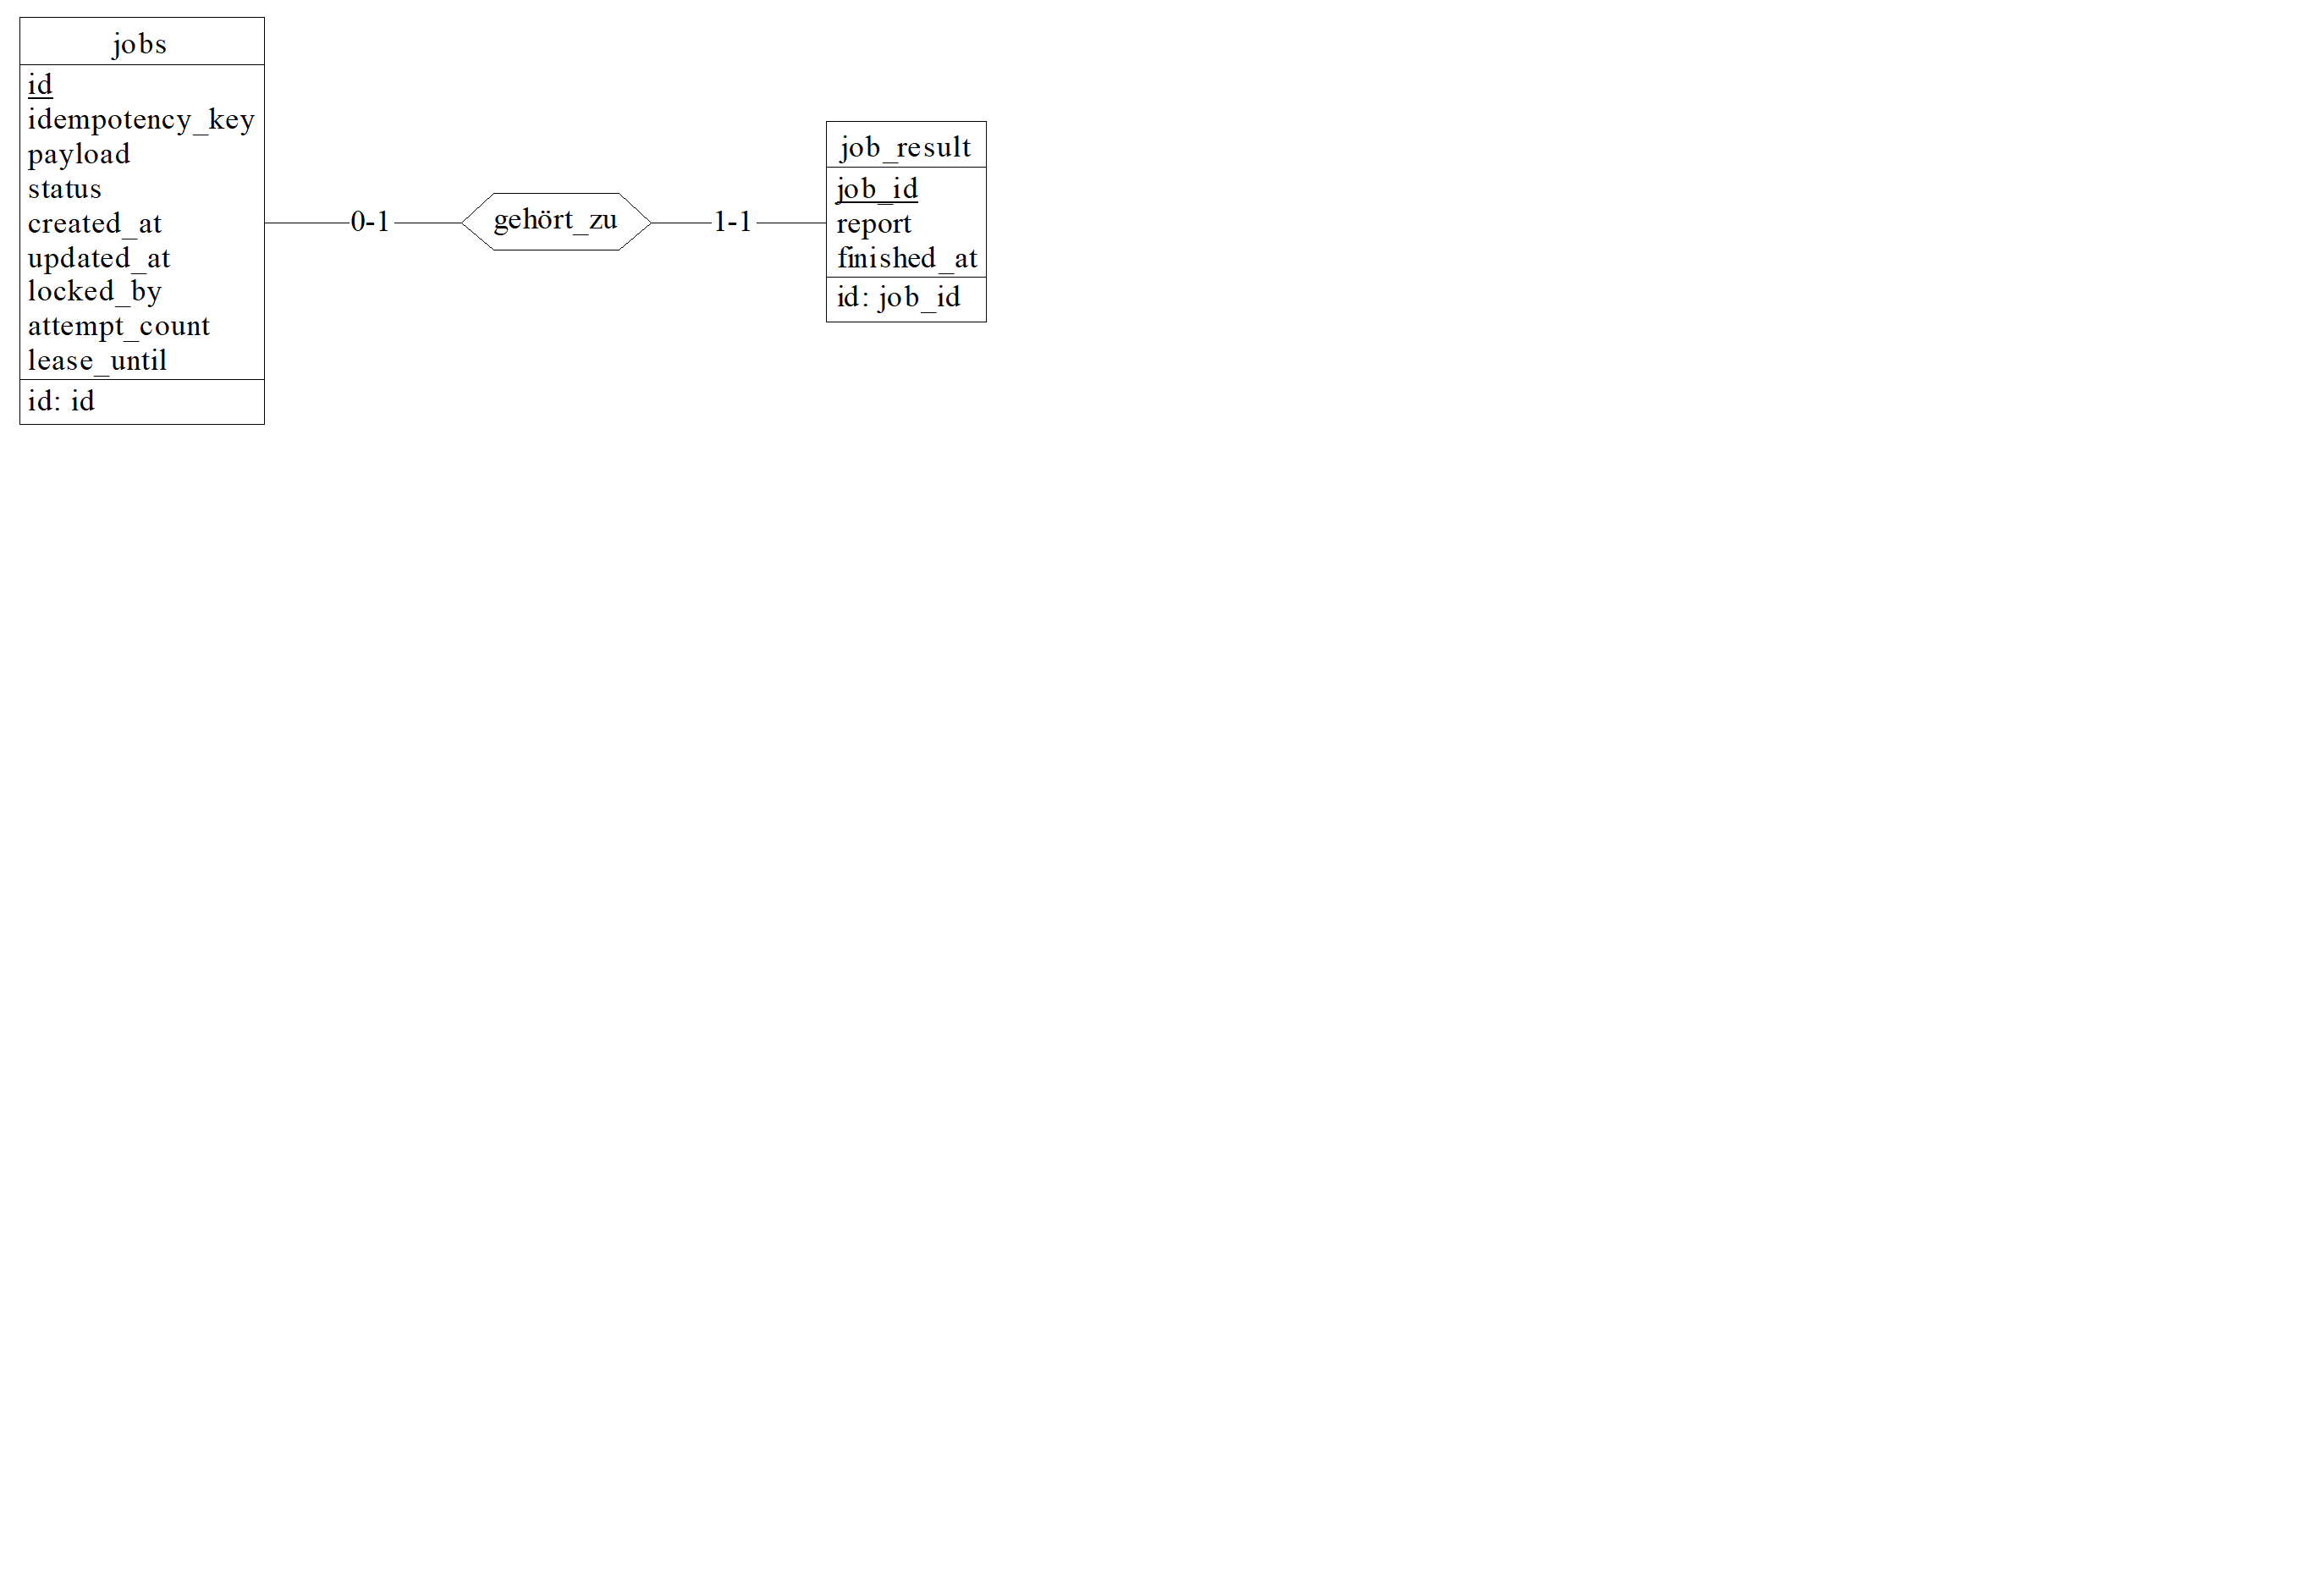
\includegraphics[width=0.8\textwidth]{images/dbSchema}
    \caption[Datenbankschema des entwickelten Job-Processing-Systems]{Datenbankschema des entwickelten Job-Processing-Systems
    mit den zur Verwaltung von Jobs, Verarbeitungszuständen und Ergebnissen verwendeten Entitäten, Attributen und ihren Beziehungen.}
    \label{fig:dbSchema}
\end{figure}

Hauptbestandteil des Schemas ist die Tabelle \texttt{jobs}.
Jeder Job besitzt zunächst einen von der Datenbank erzeugten Primärschlüssel, der zur internen Identifikation dient.
Zusätzlich wird für jeden Job ein vom Client bereitgestellter Idempotenzschlüssel gespeichert.
Damit dieser die in \ref{zus:duplikaterkennung} geforderte Idempotenz in der Joberstellung sicherstellen kann,
muss jeder Job einen eindeutigen Idempotenzschlüssel besitzen.
Daher ist die Spalte \texttt{idempotency\_key} mit einem \texttt{UNIQUE}- und einem \texttt{NOT NULL}-Constraint belegt.
Auf die Nutzung des Idempotenzschlüssels wird in \cref{subsec:joberstellung} näher eingegangen.

Neben den Identifikationsmerkmalen werden die eigentlichen Nutzdaten des Jobs als JSON-Objekt persistent gespeichert.
Dadurch kann die \textit{Payload} eine Menge an strukturierten Informationen für die Jobspezifikation beinhalten.
Alternativ könnte das Attribut auch in Abhängigkeit von der Domain und dem Systementwurf als eigene Entität
mit einer 1:1-Beziehung zum Job modelliert werden, sofern die nötigen Informationen für die Durchführung des Jobs enthalten sind.
Durch die Persistierung der Ausgangsdaten bleibt die vollständige Anfrage dauerhaft verfügbar und kann im Fehlerfall erneut verarbeitet werden,
ohne dass der Client den Job nochmals übertragen muss.
Das bildet die Grundlage für \ref{zus:verarbeitungsgarantie} und \ref{zus:idempotenz}.

Zur Umsetzung des in \cref{subsec:zustandsmodell} vorgestellten Zustandsmodells besitzt jeder Job ein Statusattribut, welches
den aktuellen Bearbeitungszustand beschreibt.
Ergänzend hierzu werden weitere Metadaten gespeichert, die für die Umsetzung der Fehlertoleranz erforderlich sind.
Das Attribut \texttt{created\_at} speichert den Zeitpunkt der Joberstellung.
Indem Worker neue Jobs in der Reihenfolge ihres Erstellungszeitpunkts beanspruchen, wird verhindert, dass ältere Jobs
dauerhaft von neu eingehenden Jobs verdrängt werden und somit im Job-Store verbleiben.
Dieses Verhalten adressiert \ref{zus:terminierung}.
Während der Bearbeitung wird im Attribut \texttt{claimed\_by} gespeichert, welcher Worker einen Job aktuell verarbeitet.
Diese Zuordnung stellt sicher, dass ausschließlich der aktuell besitzende Worker die Verarbeitung des Jobs abschließen und
das Ergebnis persistent speichern darf.
Dadurch wird die in \ref{zus:idempotenz} geforderte idempotente Ergebnisspeicherung unterstützt und verhindert, dass konkurrierende
Worker im Recovery-Fall denselben Job gleichzeitig abschließen.

Für die Recovery-Strategie wird zusätzlich die Anzahl bisheriger Bearbeitungsversuche im Attribut \texttt{attempt\_count} gespeichert.
Dadurch kann die Anzahl automatischer Wiederholungsversuche begrenzt werden, sodass fehlerhafte Jobs nicht unbegrenzt erneut ausgeführt werden.
Das Attribut \texttt{lease\_until} dient der Umsetzung zeitbasierter Leases.
Es gibt an, bis zu welchem Zeitpunkt ein Worker den beanspruchten Job exklusiv bearbeiten darf.
Überschreitet die Bearbeitung diese Zeitspanne, kann der Recovery-Service den Job als verwaist erkennen und ihn entsprechend
der definierten Recovery-Strategie erneut zur Bearbeitung freigeben.
Diese beiden Attribute werden für die Umsetzung von \ref{zus:verarbeitungsgarantie} und \ref{zus:terminierung} benötigt.

Die Verarbeitungsergebnisse werden in einer separaten Tabelle \texttt{job\_result} gespeichert.
Zwischen einem Job und seinem Ergebnis besteht dabei eine optionale Eins-zu-Eins-Beziehung.
Solange ein Job noch nicht erfolgreich bearbeitet wurde, existiert kein zugehöriger Ergebniseintrag.
Gleichzeitig darf ein Job entsprechend \ref{zus:idempotenz} höchstens ein Ergebnis besitzen.
Jedes gespeicherte Ergebnis gehört außerdem eindeutig zu genau einem Job.

Das dargestellte Datenbankschema bildet das minimale Schema zur Umsetzung der in dieser Arbeit betrachteten Fehlertoleranzmechanismen.
In realen Anwendungen kann der Job-Store beliebig um weitere fachliche Attribute oder zusätzliche Tabellen erweitert werden.
Ebenso ist es möglich, eine bereits bestehende relationale Datenbank zur Umsetzung des Job-Processing-Systems zu verwenden,
indem das vorgestellte Schema in die vorhandene Datenbank integriert wird.

\subsection{Joberstellung}
\label{subsec:joberstellung}
Die Annahme neuer Jobs im Backend gehört zur Erstellungsphase und bildet somit den Einstiegspunkt in das entwickelte Job-Processing-System.
Zur Umsetzung einer Exactly-Once Auslieferung, die aus den Zusicherungen \ref{zus:duplikaterkennung} und \ref{zus:retries} folgt,
sind verschiedene Mechanismen nötig, die im Folgenden vorgestellt werden.
Der Ablauf der Jobannahme ist in \cref{fig:jobannahme} dargestellt.

\begin{figure}[h]
    \centering
    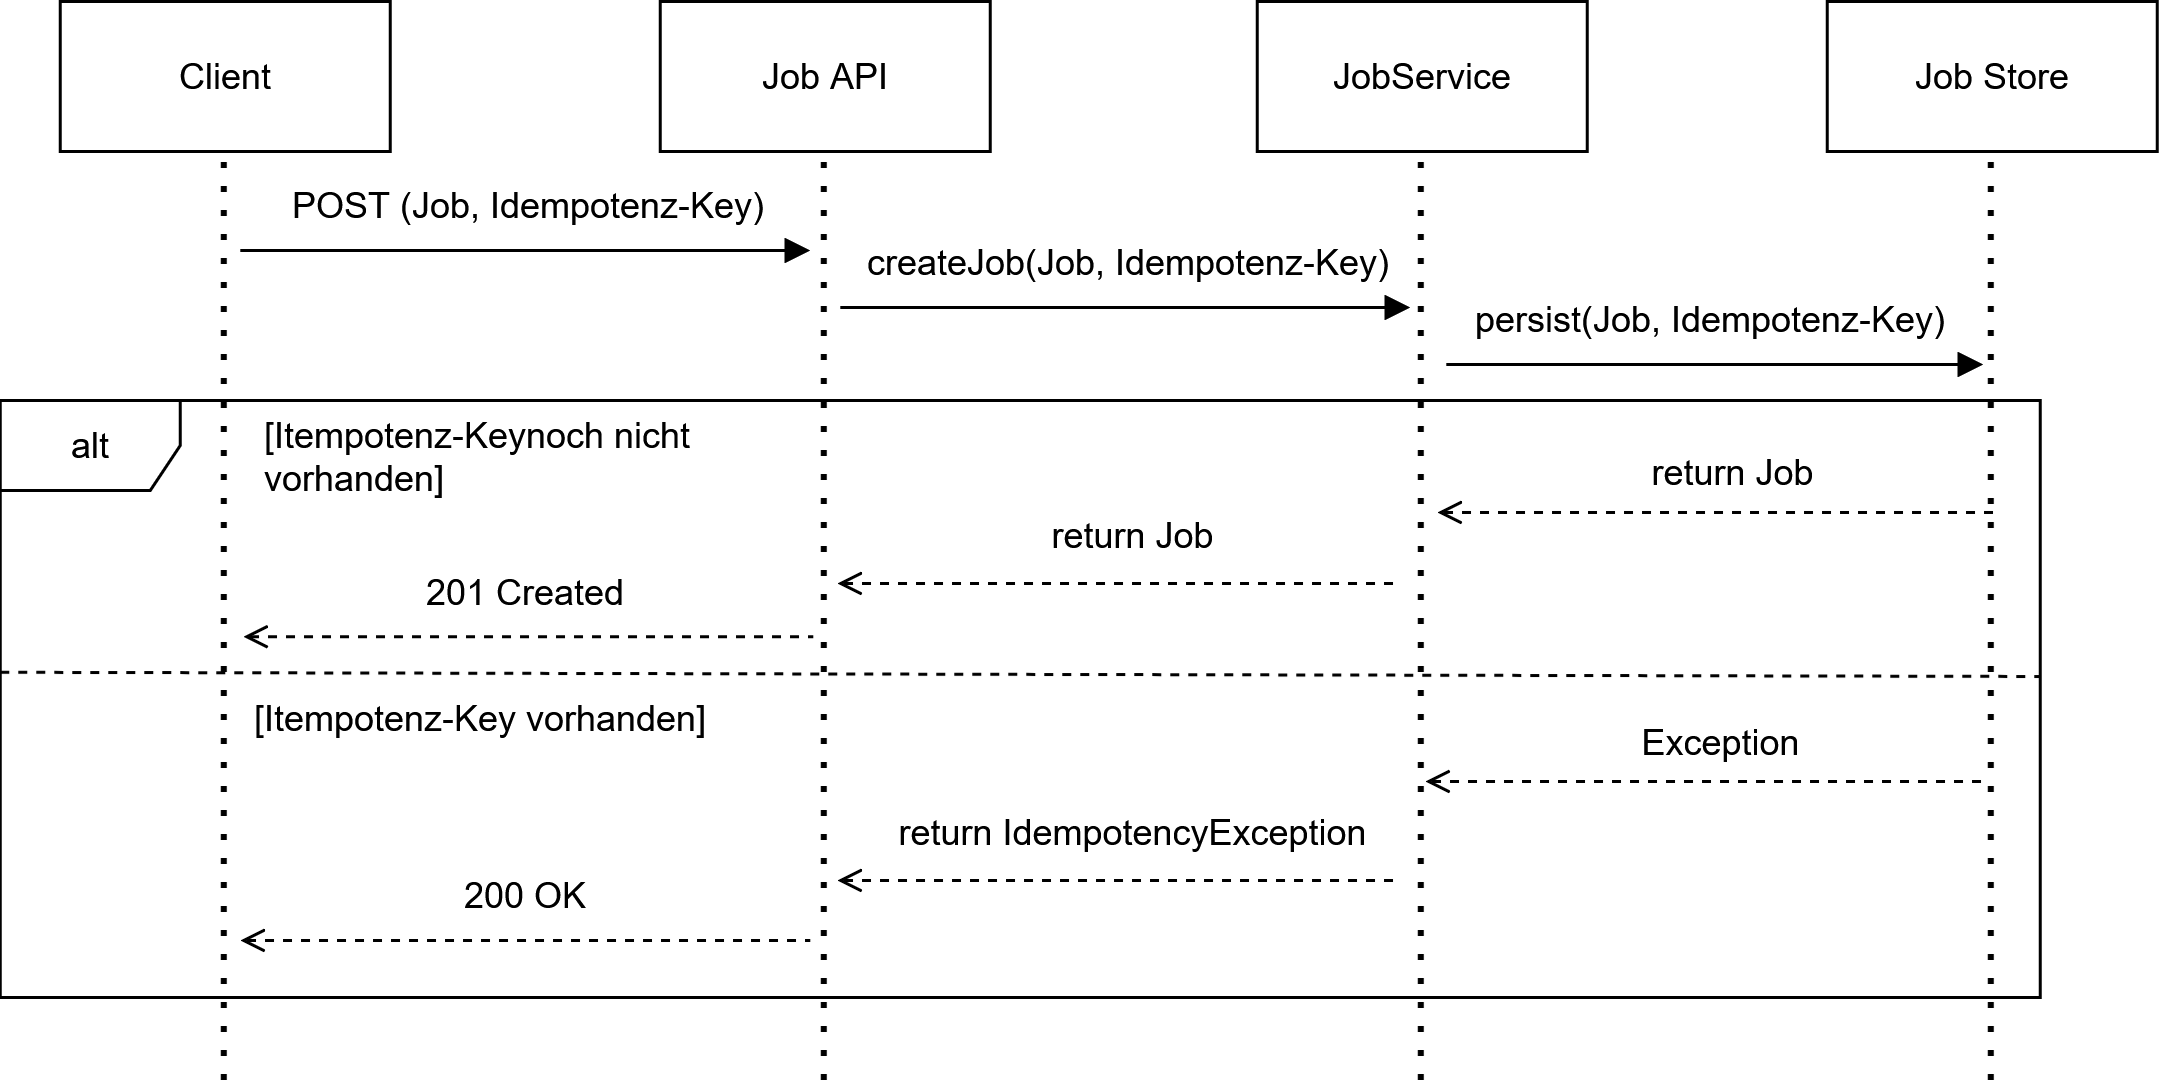
\includegraphics[width=0.95\textwidth]{images/jobannahmeSequenzdiagramm}
    \caption[Ablauf der Jobannahme]{Ablauf der Jobannahme vom Eingang einer Anfrage über die Persistierung des Jobs bis
    zur Rückgabe einer Erfolgsnachricht an den Client inklusive Unterscheidung im Duplikatsfall des Idempotenzschlüssels.}
    \label{fig:jobannahme}
\end{figure}

Zur Erstellung eines neuen Jobs sendet der Client eine Anfrage über die \gls{rest}-Schnittstelle an das Backend.
Die Anfrage besteht aus zwei Bestandteilen: der eigentlichen Nutzlast (\textit{Payload}), welche die durchzuführende Arbeit beschreibt,
sowie einem vom Client erzeugten Idempotenzschlüssel.
Dieser Schlüssel identifiziert einen Job eindeutig und ermöglicht es, mehrfach übertragene Anfragen desselben Jobs zuverlässig zu erkennen.
Die Verwendung des Idempotenzschlüssels ist insbesondere für den Fall relevant, dass der Client eine Anfrage erneut sendet,
obwohl der ursprüngliche Job bereits erfolgreich gespeichert wurde.
Ein solches Szenario kann auftreten, wenn das Acknowledgement des Backends bei der Übertragung verloren geht und der Client
deshalb fälschlicherweise von einer fehlgeschlagenen Joberstellung ausgeht.
Durch den Idempotenzschlüssel kann das Backend erkennen, dass der betroffene Job bereits existiert und eine doppelte Persistierung verhindern.
Damit wird Zusicherung \ref{zus:duplikaterkennung} umgesetzt.

Nach Eingang der Anfrage leitet der \texttt{JobController} diese an den \texttt{JobService} weiter.
Dieser versucht, den Job zusammen mit dem Idempotenzschlüssel zu speichern.
Existiert der Idempotenzschlüssel noch nicht, liefert die der Service den erstellten Job an den \texttt{JobController} zurück,
der dem Client mit dem HTTP-Statuscode \texttt{201 Created} als Bestätigung der erfolgreichen Joberstellung antwortet.
Existiert dagegen bereits ein Job mit demselben Idempotenzschlüssel, wird ein Fehler aufgrund des
\texttt{UNIQUE}-Constraints der Datenbank ausgelöst.
Dieser wird durch den Service weitergegeben und schließlich vom Controller abgefangen.
Da sich der Job bereits im System befindet und somit der gewünschte Zielzustand erreicht wurde, beantwortet der Controller
die Anfrage mit dem HTTP-Statuscode \texttt{200 OK}.

Kann während der Persistierung keine Verbindung zur Datenbank hergestellt werden oder tritt ein anderer transienter Fehler
auf, wird der Speicherversuch automatisch wiederholt.
Weitere Details zu Client- und Serverseitigen Retries werden in \cref{subsec:retryStrategie} behandelt.
Erst wenn der Job erfolgreich gespeichert wurde oder bereits existiert, wird dem Client ein erfolgreicher HTTP-Statuscode zurückgegeben.
Kann der Job dagegen auch nach Ausschöpfen aller Wiederholungsversuche nicht gespeichert werden, antwortet das Backend
mit dem HTTP-Statuscode \texttt{500 Internal Server Error}.
Dadurch kann der Client erkennen, dass kein erfolgreicher Abschluss der Operation garantiert werden konnte und den
Erstellungsversuch seinerseits gemäß der definierten Retry-Strategie wiederholen.
Dieses Zusammenspiel zwischen client- und serverseitigen Wiederholungsmechanismen stellt sicher, dass die Zusicherung \ref{zus:retries}
eingehalten wird und somit kein direktes manuelles Eingreifen nach dem ersten fehlgeschlagenen Versuch notwendig ist.

\subsection{Exklusive Verarbeitung und Transaktionsmodell}
\label{subsec:transaktionsmodell}
Wie bereits in \cref{subsec:transaktionsgrenzen} erläutert, bringen lange Transaktionen einige Nachteile mit sich.
Da Hintergrundjobs typischerweise langlaufende Berechnungen oder E/A-intensive Operationen kapseln \parencite{microsoft_corporation_hrsg_best_2026},
ist die Nutzung einer einzigen Datenbanktransaktion über den gesamten Lebenszyklus eines Jobs für dieses System nicht sinnvoll.
Anstatt den Job in einer einzelnen langlaufenden Transaktion zu verarbeiten, verfolgt das entwickelte System aus diesem Grund einen anderen Ansatz.
Die eigentliche Fachlogik wird vollständig außerhalb einer Datenbanktransaktion ausgeführt.
Datenbanktransaktionen werden ausschließlich zur atomaren Synchronisation der Zustandsübergänge verwendet und sind daher entsprechend kurz.
Die Kombination aus dem in \cref{subsec:zustandsmodell} vorgestellten Zustandsmodell und kurzlaufenden Transaktionen
ermöglicht eine exklusive Bearbeitung der Jobs, ohne Datenbankressourcen während der eigentlichen Verarbeitung zu blockieren.
Der Verarbeitungsablauf gliedert sich hierzu in drei Phasen, die in \cref{fig:transaktionsmodell} visualisiert sind.

\begin{figure}[h]
    \centering
    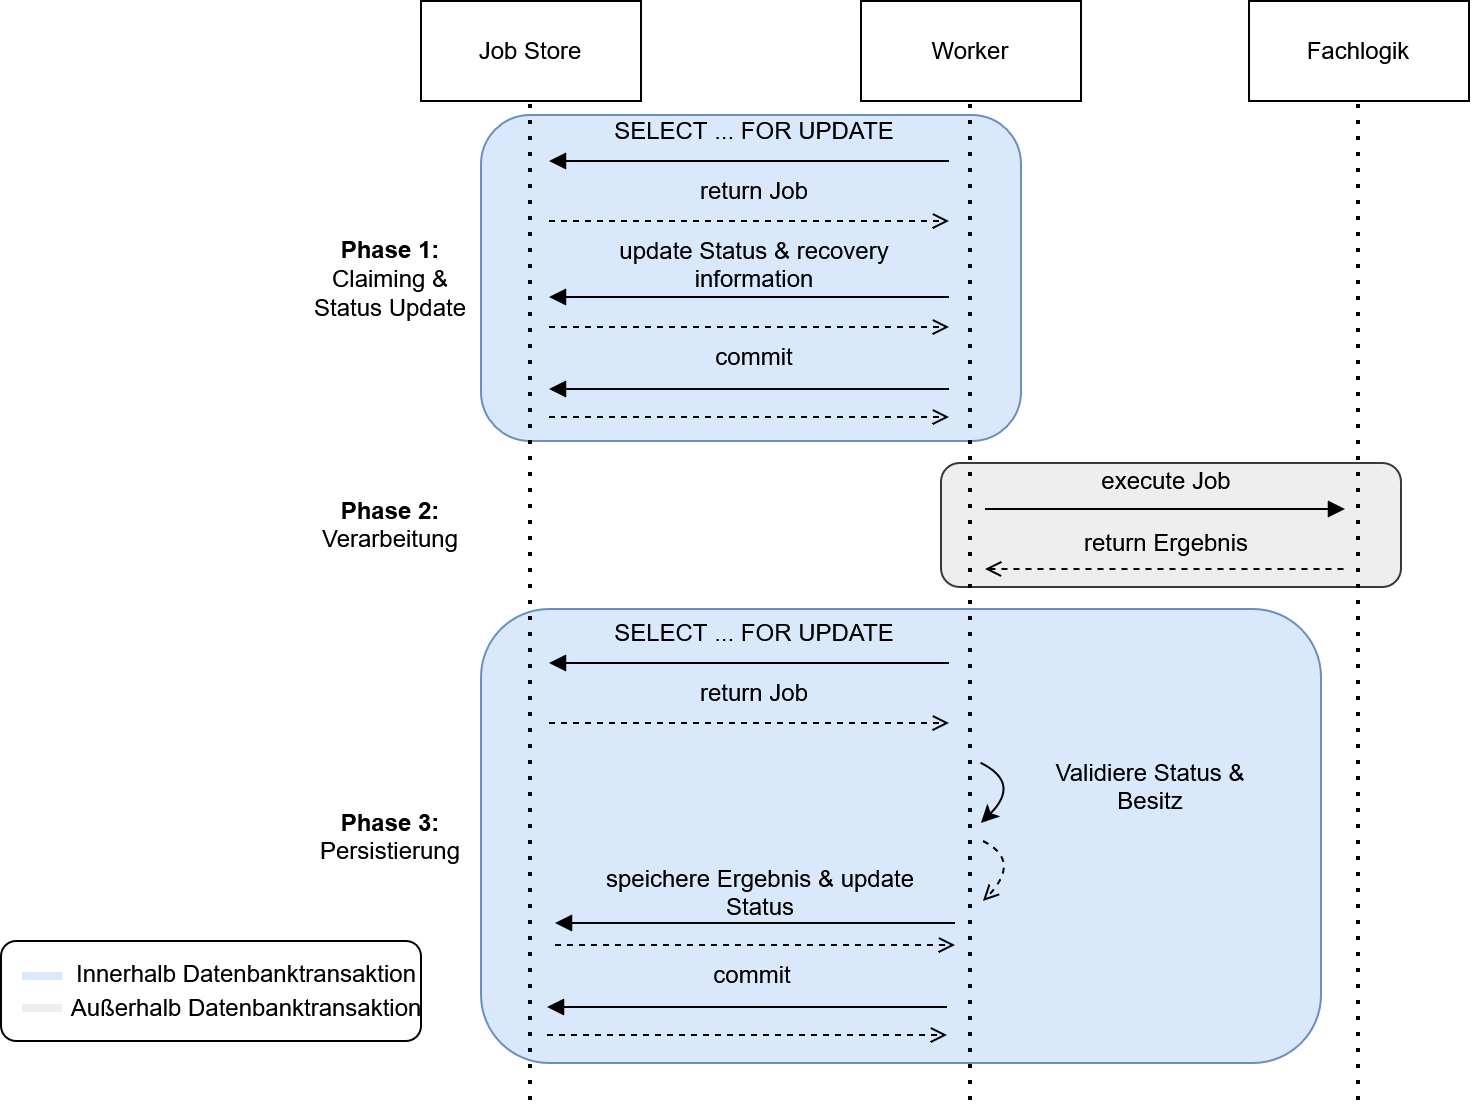
\includegraphics[width=0.9\textwidth]{images/transaktionsmodell}
    \caption[Transaktionsmodell der Jobverarbeitung]{Transaktionsmodell der Jobverarbeitung mit den Transaktionsgrenzen der
    der einzelnen Phasen des Job-Lebenszyklus und den darin ausgeführten Operationen.}
    \label{fig:transaktionsmodell}
\end{figure}

Zunächst beansprucht ein Worker innerhalb einer Datenbanktransaktion einen freien Job.
Hierzu wird mittels \texttt{SELECT~…~FOR~UPDATE~SKIP~LOCKED} ein geeigneter Job ausgewählt und exklusiv gesperrt.
Dadurch wird nicht auf bereits von anderen Workern reservierte Jobs blockierend gewartet, sondern diese werden unmittelbar übersprungen.
Zusätzlich wird der Jobstatus von \textit{Queued} nach \textit{Running} überführt und die Attribute für die Recovery wie
\texttt{claimed\_by}, \texttt{attempt\_count} oder \texttt{lease\_until} werden aktualisiert.
Unmittelbar nach diesen Änderungen wird die Transaktion committet und die Datenbankverbindung wieder freigegeben.
Anschließend erfolgt die eigentliche Verarbeitung des Jobs vollständig außerhalb einer Datenbanktransaktion.
Da der Job bereits den Zustand \textit{Running} besitzt, können andere Worker ihn währenddessen nicht erneut beanspruchen.
Nach erfolgreichem Abschluss der eigentlichen Fachlogik wird zunächst eine neue Transaktion geöffnet.
Dort wird geprüft, ob der Worker noch immer die Speicherberechtigung für den Job besitzt.
Falls ja, wird sowohl das Verarbeitungsergebnis persistent gespeichert als auch der Jobstatus von \textit{Running} auf
\textit{Succeeded} aktualisiert.
Beide Änderungen werden gemeinsam committet.
Dadurch ist sichergestellt, dass niemals ein Zustand entstehen kann, in dem zwar bereits ein Ergebnis gespeichert wurde,
der Job jedoch weiterhin als \textit{Running} gekennzeichnet ist oder der Job als \textit{Succeeded} markiert ist, aber kein
Ergebnis gespeichert wurde.
Die gemeinsame Speicherung von Ergebnis und Jobstatus innerhalb derselben lokalen Transaktion gewährleistet
somit durch die \gls{acid}-Garantien die in \ref{zus:atomare_wirkung} geforderte Atomarität.
Somit wird die Konsistenz der Daten gewahrt, indem sämtliche Änderungen am Job vor parallelen Zugriffen und Fehlern geschützt werden,
während die eigentliche Fachlogik vollständig außerhalb der Transaktionsgrenzen verbleibt.

Für die Synchronisation konkurrierender Worker wird ein pessimistisches Sperrverfahren verwendet.
Wie bereits in \cref{subsec:synchronisation} erläutert, eignen sich optimistische Synchronisationsverfahren insbesondere
für Systeme, in denen konkurrierende Änderungen nur selten auftreten.
Im entwickelten Job-Processing-System ist jedoch das Gegenteil der Fall.
Da alle Worker neue Jobs entsprechend ihres Erstellungszeitpunkts aus derselben Warteschlange entnehmen, konkurrieren sie
regelmäßig um dieselben Datensätze.
Optimistische Verfahren würden in diesem Szenario zu einer hohen Anzahl abgebrochener Transaktionen und entsprechender Wiederholungsversuche führen.
\textcite[Kap.~7 Abschnitt \glqq Pessimistic versus optimistic concurrency control\grqq]{kleppmann_designing_2017}
weist darauf hin, dass sich optimistische Verfahren bei hoher Konkurrenz negativ auf den Gesamtdurchsatz auswirken,
da die zusätzlich notwendigen Wiederholungen die Datenbank weiter belasten.
Aus diesem Grund wird im Rahmen dieser Arbeit ein pessimistisches Sperrverfahren verwendet, bei dem konkurrierende
Zugriffe bereits während der Auswahl eines Jobs verhindert werden.
Durch die Nutzung expliziter Sperren wird die exklusive Bearbeitung unabhängig vom verwendeten Isolation Level gewährleistet.
Aus diesem Grund genügt das in PostgreSQL standardmäßig verwendete Isolation-Level READ COMMITTED, da die notwendige Synchronisation
durch die expliziten Sperren erfolgt und strengere Isolationsebenen für den beschriebenen Ablauf keinen zusätzlichen Nutzen bieten.

\subsection{Retry-Strategie}
\label{subsec:retryStrategie}
Auf Grundlage der in \cref{subsec:retry/backoff} beschriebenen Prinzipien werden Wiederholungsmechanismen gezielt an denjenigen
Stellen der Architektur eingesetzt, an denen temporäre Infrastrukturfehler auftreten können.
Ziel ist es im Rahmen von \ref{zus:retries}, kurzfristige Störungen durch Wiederholungsversuche zu kompensieren und
dadurch unnötige Recovery-Vorgänge oder Benutzerinteraktionen zu vermeiden.
Hierzu unterscheidet die Architektur zwischen der Kommunikation des Clients mit dem Backend und den internen
Datenbankzugriffen durch die Worker und den \texttt{JobController}.
Beide Kommunikationswege stellen voneinander unabhängige Fehlerquellen dar und können daher unabhängig voneinander von
transienten Infrastrukturfehlern betroffen sein.

Auf Clientseite werden Wiederholungsversuche für die Kommunikation mit der \gls{rest}-Schnittstelle des Backends vorgesehen.
Kann eine Anfrage aufgrund einer temporären Netzwerkstörung oder einer kurzfristigen Nichtverfügbarkeit des Backends
nicht erfolgreich abgeschlossen werden beziehungsweise bleibt die Erfolgsbestätigung aus, wird die Anfrage automatisch erneut übertragen.
Da die Joberstellung durch den in \cref{subsec:joberstellung} beschriebenen Idempotenzmechanismus abgesichert ist,
kann eine erneute Übertragung derselben Anfrage nicht zu einer mehrfachen Persistierung eines Jobs führen.
Die Kombination aus Retry und Idempotenz schafft somit eine Exactly-Once-Semantik für die Joberstellung unter der Voraussetzung,
dass der Fehler tatsächlich transient ist und die Parameter für Retry und Backoff passend konfiguriert sind.

Auch innerhalb des Backends werden Wiederholungsversuche für Datenbankzugriffe vorgesehen, deren Fehlschlagen
auf transiente Infrastrukturfehler zurückzuführen ist.
Dazu zählt unter anderem auch die temporäre Nichtverfügbarkeit der Datenbank.
Kann eine Operation aufgrund eines solchen Fehlers nicht abgeschlossen werden, wird sie automatisch erneut ausgeführt.

Fachliche Fehler während der eigentlichen Jobverarbeitung werden bewusst nicht wiederholt, da deren Ursache nicht
durch einen erneuten Ausführungsversuch beseitigt werden kann.

Zur strukturellen Entkopplung der Wiederholungslogik wird diese in einer eigenständigen Retry-Komponente gekapselt.
Wie in \cref{fig:retryClassDiagram} dargestellt, nutzen die jeweiligen Komponenten, wie der Client im Frontend
zur Erstellung der Jobs, einen zentralen \texttt{RetryExecutor}, der die auszuführende Operation über die Methode \textit{execute(...)}
entgegennimmt und deren Ausführung entsprechend einer konkreten \texttt{RetryPolicy} steuert.

\begin{figure}[h]
    \centering
    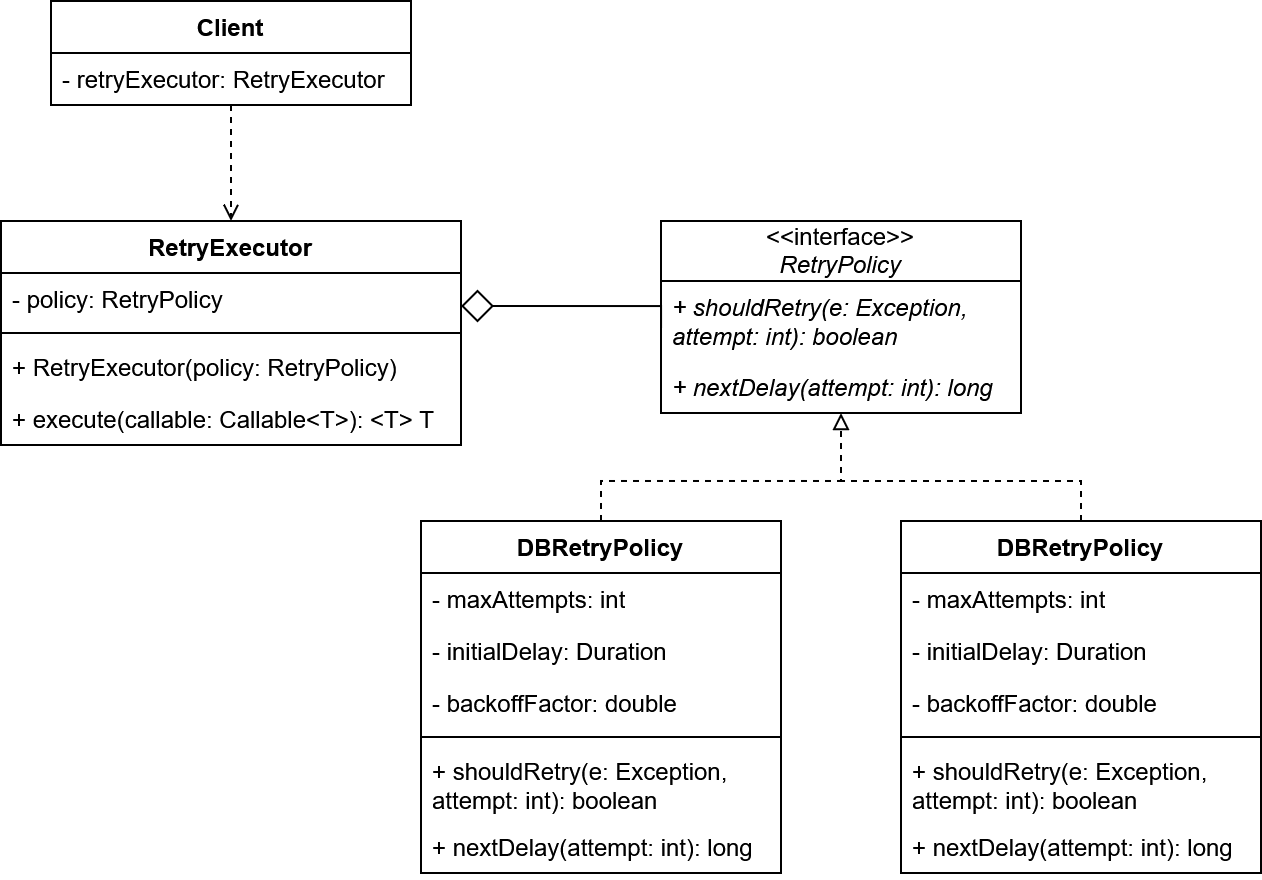
\includegraphics[width=0.8\textwidth]{images/retryClassDiagramm}
    \caption[Klassendiagramm der Retry-Komponente]{Klassendiagramm der Retry-Komponente mit dem Retry-Executor als Schnittstelle
    für den Client inklusive der Konfiguration durch unterschiedliche Policies.}
    \label{fig:retryClassDiagram}
\end{figure}

Der RetryExecutor enthält dabei selbst keine anwendungsspezifischen Entscheidungen darüber, wann eine Wiederholung erfolgen soll.
Stattdessen fängt er Exceptions von der auszuführenden Operation und gibt sie an \textit{shouldRetry(...)} weiter.
Die spezifische Policy entscheidet dann, ob ein Retry sinnvoll ist oder nicht, indem sie die Exception klassifiziert und einen
entsprechenden Wahrheitswert zurückliefert.
Die Retry-Policies implementieren dabei eigene unterschiedliche Kriterien für Wiederholungsversuche, die sich in den behandelten
Fehlerarten unterscheiden.
Außerdem definieren sie über \textit{nextDelay(...)}, wie das Backoff-Verhalten umgesetzt wird.
Für das Job-Processing-System wird dabei ein exponentielles Backoff verwendet.
Wie in \cref{subsec:retry/backoff} beschrieben, verhindert das die zusätzliche Belastung bereits beeinträchtigter Systeme.
Die Verzögerung ergibt sich dabei aus
\[
    d_n = d_0 \cdot b^{\,n-1},
\]
wobei $d_n$ die Wartezeit des aktuellen Wiederholungsversuchs, $d_0$ die initiale Wartezeit, $b$ den Backoff-Faktor und
$n$ die Nummer des aktuellen Wiederholungsversuchs bezeichnet.
Mit jedem weiteren Fehlversuch vergrößert sich somit das Warteintervall exponentiell.

Durch die Nutzung eines solchen Strategy-Patterns kann dieselbe Retry-Komponente sowohl für die Kommunikation zwischen
Client und Backend als auch für backendseitige Datenbankzugriffe verwendet werden, obwohl sich die jeweils
behandelten Fehlerarten unterscheiden.
Die Retry-Steuerung bleibt dadurch zentral gekapselt, während die konkrete Fehlerbehandlung an den jeweiligen
Anwendungskontext angepasst werden kann.
Die konkrete Implementierung des \texttt{RetryExecutor} sowie die Konfiguration der einzelnen Retry-Policies werden in
\cref{subsec:impl_retries} erläutert.

\subsection{Recovery}
\label{subsec:recoveryarchitektur}
Die in \cref{subsec:retryStrategie} beschriebene Retry-Strategie behandelt ausschließlich transiente Infrastrukturfehler,
bei denen die ausführende Komponente weiterhin aktiv ist.
Fällt ein Worker dagegen während der Verarbeitung vollständig aus oder bleibt dauerhaft hängen, kann kein lokaler Retry mehr erfolgen.
Zur Behandlung solcher Fehler wird die Architektur daher um einen eigenständigen Recovery-Service ergänzt.
Dieser überprüft den Job-Store in regelmäßigen Abständen auf potenziell verwaiste Jobs.
Hierzu werden sämtliche Jobs betrachtet, die sich weiterhin im Zustand \textit{Running} befinden, deren Lease jedoch bereits abgelaufen ist.
Die Architektur verzichtet im Rahmen der Prototypentwicklung bewusst auf einen Heartbeat-Mechanismus und nutzt stattdessen
zeitbasierte Leases, da diese ohne zusätzliche Kommunikation zwischen Worker und Job-Store auskommen.
Dies belastet die Datenbank weniger und reduziert gleichzeitig den Implementierungsaufwand.
Da der Prototyp nur eine simulierte Fachlogik mit festgelegter Jobdauer nutzt, fänden die Vorteile von Heartbeats hier keine Anwendung.
Daraus resultierende Konsequenzen werden in \cref{sec:einschraenkungen} diskutiert.
Für ein Produktivsystem ist die Nutzung eines Heartbeat-Mechanismus aber durchaus legitim und unter Umständen sogar sinnvoll.

Für jeden erkannten verwaisten Job entscheidet der Recovery-Service anschließend über das weitere Vorgehen.
Wurde die maximal zulässige Anzahl an Ausführungsversuchen noch nicht erreicht, werden innerhalb einer zusammengehörigen
Transaktion der Status auf \textit{Queued} sowie die Attribute \texttt{claimed\_by} und \texttt{lease\_until} zurückgesetzt.
Anschließend kann der Job von einem beliebigen Worker erneut beansprucht werden.
Wurde die konfigurierte Obergrenze der Wiederholungsversuche bereits erreicht, wird der Job stattdessen in den
Endzustand \textit{Failed} überführt und nicht erneut verarbeitet.
Dadurch wird verhindert, dass dauerhaft fehlerhafte Jobs unbegrenzt Systemressourcen belegen und nie terminieren (\ref{zus:terminierung}).
Durch diesen Mechanismus können insbesondere Worker-Abstürze, JVM-Abstürze, Container-Neustarts sowie dauerhaft blockierte
Worker in Bezug auf die Jobausführung behandelt werden (\ref{zus:verarbeitungsgarantie}).
Die eigentliche Terminierung oder der Neustart fehlerhafter Worker ist dagegen nicht Bestandteil des entwickelten Systems.
Diese Aufgabe wird bewusst an eine externe Prozessüberwachung oder Orchestrierungsplattform, beispielsweise Kubernetes, delegiert.
Das entwickelte System stellt lediglich sicher, dass durch den Ausfall eines Workers kein Job dauerhaft verloren geht oder hängen bleibt.

Die Wiederaufnahme eines Jobs erfolgt in der entwickelten Architektur grundsätzlich nicht durch das Fortsetzen eines
unterbrochenen Jobs, sondern durch eine vollständige Neuausführung auf Basis der ursprünglich persistierten Eingabedaten.
Aus diesem Grund muss die Payload eines Jobs mindestens bis zum erfolgreichen Abschluss unverändert im Job-Store verbleiben.
Dadurch kann jeder Wiederholungsversuch unter identischen Ausgangsbedingungen beginnen und unvollständig abgeschlossene
Ausführungsversuche haben keine Auswirkungen auf den Erfolg oder das Ergebnis späterer Wiederholungen (\ref{zus:idempotenz}).
Problematisch ist ein solches Vorgehen jedoch, wenn während der Verarbeitung externe Seiteneffekte entstehen.
Wird beispielsweise wie in der schematischen Darstellung aus \cref{fig:seiteneffekte} im Rahmen eines Jobs eine E-Mail versendet
und der Worker stürzt anschließend vor dem erfolgreichen Abschluss der Verarbeitung ab, so wird der Job durch den
Recovery-Service erneut zur Verarbeitung freigegeben.
Die erneute Ausführung würde in diesem Fall dieselbe E-Mail ein weiteres Mal versenden.

\begin{figure}[h]
    \centering
    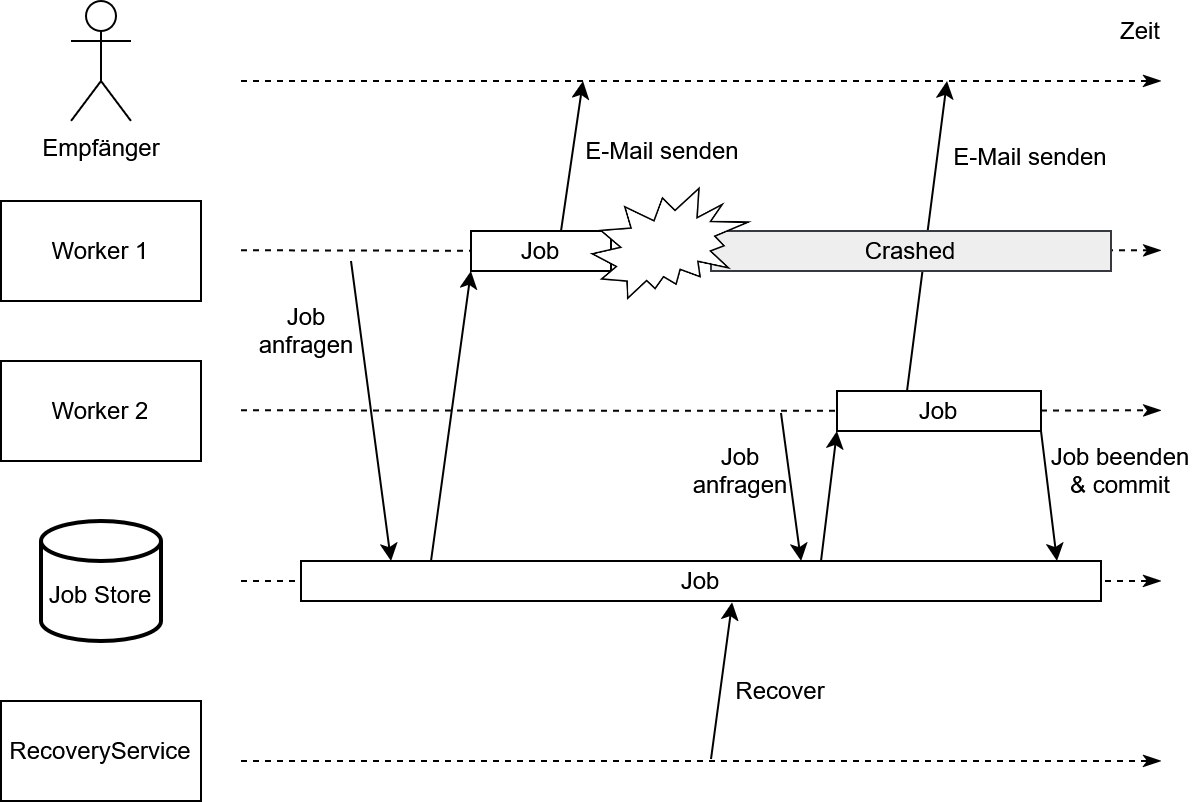
\includegraphics[width=0.9\textwidth]{images/wiederholungenBeiSeiteneffekten}
    \caption[Mehrfachausführung einer Operation mit Seiteneffekten]{Problematik einer nach einem Crash wiederholt
    ausgeführten Operation mit Seiteneffekten: Durch Neustart eines abgebrochenen Jobs kann die Wiederaufnahme
    zur ungewollten Mehrfachausführung einer Operation führen.}
    \label{fig:seiteneffekte}
\end{figure}

Die entwickelte Infrastruktur garantiert daher ausschließlich die idempotente Verarbeitung der internen Fachlogik des Job-Processing-Systems.
Für externe Seiteneffekte kann eine Exactly-Once-Ausführung dagegen grundsätzlich nicht gewährleistet werden.
Wie schon in \cref{subsec:exactlyOnce} erwähnt ist dies nur möglich, wenn das jeweils aufgerufene Zielsystem selbst eine
idempotente Verarbeitung unterstützt, beispielsweise durch Nutzung von Idempotenzschlüsseln wie im Beispielsystem bei
der Joberstellung (vgl. \cref{subsec:joberstellung}).
Unterstützt das Zielsystem keine entsprechende Semantik, kann eine Mehrfachausführung von Seiteneffekten infolge eines
Recovery-Vorgangs nicht ausgeschlossen werden.

Ein Nebeneffekt der entworfenen Architektur besteht darin, dass ein Job zeitweise von mehreren Workern gleichzeitig bearbeitet werden kann.
Überschreitet ein Worker seine Lease-Dauer, wird der Job erneut freigegeben, obwohl der ursprüngliche Worker
seine Verarbeitung möglicherweise noch beendet.
Die Strategie verfolgt damit das Ziel einer At-least-Once-Ausführung von Jobs, erzeugt damit aber die Möglichkeit der Mehrfachausführung.
Die daraus resultierenden Anforderungen an die idempotente Verarbeitung werden im folgenden Abschnitt betrachtet.

\subsection{Idempotente Ergebnisgenerierung}
\label{subsec:idempotenteErgebnisgenerierung}
\ref{zus:idempotenz} verlangt, dass pro Job maximal ein Ergebnis erzeugt wird.
Das in \cref{subsec:transaktionsmodell} vorgestellte Claiming-Verfahren stellt sicher, dass ein Job im Normalfall
ausschließlich von einem einzelnen Worker bearbeitet wird.
Durch den in \cref{subsec:recoveryarchitektur} genauer betrachteten Recovery-Fall kann diese Eigenschaft jedoch nicht immer garantiert werden.
Daher muss sichergestellt werden, dass das fachliche Ergebnis nur einmal gespeichert werden kann oder die Fachlogik auch bei
mehrfacher Ausführung in jedem Fall immer das gleiche Ergebnis erzeugt.
Da der Jobstatus sowie die Jobergebnisse in derselben Datenbank verwaltet werden, bietet sich die Umsetzung der ersten
Option mithilfe von Transaktionen an.
Um die idempotente Verarbeitung auf diese Weise sicherzustellen, darf ein Worker ein Verarbeitungsergebnis ausschließlich
dann persistent speichern, wenn er laut Job-Store weiterhin der Besitzer des Jobs ist und für den Job noch kein Ergebnis vorliegt.
Vor der Speicherung wird daher der betroffene Datensatz gesperrt und innerhalb einer transaktional geschützten Operation
erneut der aktuelle Jobstatus, die Worker-ID sowie die Gültigkeit des Leases überprüft.
Nur wenn der Job sich weiterhin im Zustand \textit{Running} befindet, die gespeicherte Worker-ID mit der des ausführenden Workers
übereinstimmt und das Lease noch nicht abgelaufen ist, wird das Ergebnis übernommen und der Job erfolgreich abgeschlossen.
Andernfalls wird der Speichervorgang verworfen, da bereits ein anderer Worker die weitere Verarbeitung übernommen hat, das
Lease abgelaufen ist oder der Job bereits abgeschlossen oder recovered wurde.
Dieses Prinzip wird auch \textit{\enquote{Fencing}} \parencite[Kap.~8 Abschnitt \glqq Fencing tokens\grqq]{kleppmann_designing_2017} genannt.
Dadurch kann jeder Job höchstens einmal erfolgreich gespeichert werden, selbst wenn mehrere Worker denselben Job parallel ausgeführt haben.
Das in \cref{subsec:recoveryarchitektur} bereits erwähnte Problem bezüglich Seiteneffekten in externen Systemen bleibt jedoch bestehen.


\section{Implementierung}
\label{sec:implementierung}
Die sich aus \ref{item:tz3} ergebende Implementierung des Systems orientiert sich unmittelbar an dem in \cref{sec:architektur}
erarbeiteten Systementwurf zur Umsetzung der definierten Zusicherungen.
Das Kapitel gliedert sich wie folgt:
\cref{subsec:technologien} begründet zunächst die Auswahl der verwendeten Technologien.
In \cref{subsec:impl_persistenz} wird die datenbankseitige Abbildung der Entitäten sowie die Kapselung der SQL-Zugriffe im Repository behandelt.
\cref{subsec:impl_joberstellung} erläutert den Aufbau und Ablauf der Joberstellung, woraufhin
\cref{subsec:impl_verarbeitung} die Komponenten zur Verarbeitung der Jobs beschreibt.
Der atomare Abschluss von Jobs und die Absicherung gegen fehlerhafte Doppelverarbeitungen wird in
\cref{subsec:impl_abschlussJoberverarbeitung} dargelegt.
Schließlich widmet sich \cref{subsec:impl_retries} der konkreten Umsetzung des Retry-Mechanismus und \cref{subsec:impl_recovery}
der Wiederherstellung verwaister Jobs.
Eine detaillierte Bausteinsicht der Backend-Komponente ist in \cref{fig:detailBausteinsicht} im Anhang zu finden und
dient im Folgenden als Referenz für die Beschreibung der Implementierung.

\subsection{Auswahl verwendeter Technologien}
\label{subsec:technologien}
Die Implementierung des entwickelten Background-Job-Processing-Systems erfolgt vollständig in Java.
Wie bereits ausführlich in \cref{subsec:architekturentwurf} begründet, wird PostgreSQL dabei als zentraler Job-Store verwendet.
Als Entwicklungsplattform wird das Spring-Framework in Kombination mit Spring Boot eingesetzt, da dieses eine umfangreiche
Infrastruktur für den Aufbau transaktionsbasierter Client-Server-Anwendungen bereitstellt und gleichzeitig viele der im
Architekturentwurf vorgesehenen Mechanismen direkt unterstützt.
Darüber hinaus zählt Spring zu einem etablierten Framework für die Entwicklung von Java-Backend-Anwendungen.
Dadurch entsteht eine praxisnahe Technologiebasis, die gleichzeitig einen hohen Grad an Automatisierung bietet.
Die wichtigsten verwendeten Spring-Komponenten sind in \cref{tab:technologieStack} aufgelistet.
Die bereitgestellten Framework-Funktionen reduzieren den Implementierungsaufwand für Infrastrukturaufgaben und ermöglichen
es, den Fokus auf die Entwicklung und Evaluation der im Architekturentwurf beschriebenen Mechanismen zu legen.
\begin{table}[h]
    \centering
    \begin{tabularx}{\textwidth}{llX}
        \toprule
        \textbf{Funktion} & \textbf{Komponente} & \textbf{Begründung}\\
        \midrule
        \gls{rest}-Schnittstelle & Spring Web & Bereitstellung und Nutzung der HTTP-Endpunkte und (De-)\allowbreak{}Serialisierung von JSON\\ %TODO: brauche ich HTTP und JSON als Abkürzung?
        Datenbankzugriff & Spring Data JPA & Bereitstellung von Standardoperationen und Abstraktion\\
        Transaktionale Kapselung & Spring Transactions & Ermöglicht Definition eigener Transaktionsgrenzen\\
        \bottomrule
    \end{tabularx}
    \caption[Übersicht der Spring-Komponenten]{Übersicht der wichtigsten im Rahmen der Arbeit genutzten Spring-Komponenten zur Implementierung
    des Prototyps.}
    \label{tab:technologieStack}
\end{table}

\subsection{Persistenz und Datenbankzugriff}
\label{subsec:impl_persistenz}
Die Abbildung der persistenten Daten erfolgt durch die Entitätsklassen \texttt{Job} und \texttt{JobResult}, die jeweils mit
der Annotation \texttt{@Entity} versehen sind.
Der Status eines Jobs wird als Java-Enumeration modelliert und über JPA persistent gespeichert.
Damit wird sichergestellt, dass ausschließlich die im Zustandsmodell definierten Zustände verwendet werden können.

Eine besondere Bedeutung besitzt der Idempotenzschlüssel.
Dieser wird vom Client als \texttt{\gls{uuid}} erzeugt und dient zur Erkennung mehrfach übermittelter Anfragen.
Die Umsetzung der in \cref{subsec:datenbankentwurf} definierten Constraints wird über \texttt{@Column(nullable = false, unique = true)}
umgesetzt und stellt somit die Eindeutigkeit erstellter Jobs auf Datenbankebene sicher (\ref{zus:duplikaterkennung}).

Die Verarbeitungsergebnisse werden durch die Entitätsklasse \texttt{JobResult} repräsentiert.
Umgesetzt wird die 1:1-Beziehung zwischen \texttt{JobResult} und \texttt{Job} über die \texttt{@OneToOne}-Annotation.
Dabei wird die Fremdschlüsselbeziehung über \texttt{@JoinColumn} in der Tabelle des Ergebnisses umgesetzt.
Die Beschränkung auf höchstens ein Ergebnis pro Job ist insbesondere für die idempotente Ergebnisspeicherung relevant (\ref{zus:idempotenz}).
Daher wird auch der Fremdschlüssel des \texttt{JobResult} mit einem \texttt{UNIQUE}-Constraint belegt.

Ein Repository-Interface kapselt den Datenbankzugriff und definiert neben den von JPA bereitgestellten Standardoperationen
weitere spezifische Abfragen, die unmittelbar die Anforderungen an die konkurrierende Verarbeitung und die Recovery unterstützen.
Für die Auswahl eines Jobs zur Verarbeitung wird beispielsweise die in \cref{lst:claiming} dargestellte native SQL-Abfrage definiert.

\begin{lstlisting}[
    language=SQL,
    style=sql,
    caption={[Auswahl und Sperrung eines Jobs zur Verarbeitung]{Auswahl einer übergebenen Anzahl verfügbarer Jobs anhand seines Zustands
    und Erstellungszeitpunkts sowie exklusive Sperrung der ausgewählten Datensätze mittels \texttt{FOR UPDATE SKIP LOCKED}.}},
    label={lst:claiming}
]
SELECT *
FROM jobs
WHERE status = :status
ORDER BY created_at
LIMIT :limit
FOR UPDATE SKIP LOCKED
\end{lstlisting}

Beim Aufruf der Anfrage wird sie mit einem Status und einer Anzahl parametrisiert und liefert maximal die übergebene Anzahl
Datensätze zurück, die sich im übergebenen Zustand befinden.
Die Sortierung nach dem Erstellungszeitpunkt stellt dabei sicher, dass ältere Jobs bevorzugt verarbeitet werden (\ref{zus:terminierung}).
\texttt{FOR UPDATE} sperrt dabei den ausgewählten Datensatz für die laufende Transaktion zum Zweck des exklusiven Zugriffs
(\ref{zus:exklusive_rechte}), während \texttt{SKIP LOCKED} bereits durch andere Transaktionen gesperrte Datensätze ignoriert.
Dadurch können mehrere Worker gleichzeitig nach verfügbaren Jobs suchen, ohne sich gegenseitig durch gesperrte Datensätze
zu blockieren.

Für den Abschluss einer Verarbeitung und Recovery-Szenarien wird der in \cref{lst:forUpdate} gezeigte Befehl
zum gezielten Zugriff auf einzelne Jobs bereitgestellt, der mit der Auswahl eine Sperre für diesen Datensatz setzt.

\begin{lstlisting}[
    language=SQL,
    style=sql,
    caption={[Exklusives Laden eines Jobs zur Bearbeitung]{Exklusives Laden eines Jobs zur Bearbeitung anhand seiner
    ID. Dabei wird der zugehörige Datensatz für die Dauer der laufenden Transaktion mittels \texttt{FOR UPDATE} gesperrt.}},
    label={lst:forUpdate}
]
SELECT *
FROM jobs
WHERE id = :jobId
FOR UPDATE
\end{lstlisting}

Auch dieser Befehl dient dazu, konkurrierende Änderungen an einem konkreten Job zu verhindern (\ref{zus:exklusive_rechte}).

Zusätzlich stellt das Repository eine Abfrage bereit, mit der Jobs anhand der Kombination ihres Status und des Ablaufs ihres Leases
identifiziert werden können.
Damit bildet die Abfrage aus \cref{lst:verwaisteJobs} die Grundlage für die Erkennung verwaister Jobs durch den Recovery-Mechanismus.

\begin{lstlisting}[
    language=SQL,
    style=sql,
    caption={[Identifikation verwaister Jobs]{Identifikation von Jobs anhand des Zustands und des Ablaufzeitpunkts des
    Leases als Grundlage für die Recovery.}},
    label={lst:verwaisteJobs}
]
SELECT j.id
FROM Job j
WHERE j.status = :status
AND j.lease_until < :timestamp
\end{lstlisting}

Wird der gesuchte Status auf \textit{Running} und der \texttt{timestamp} auf den aktuellen Zeitpunkt gesetzt, liefert
die Anfrage die ID aller Jobs, die noch nicht beendet wurden und deren Lease zusätzlich abgelaufen ist.

Die Transaktionskapselung wird durch \texttt{@Transactional} erreicht.
Alle Datenbankoperationen in einer mit \texttt{@Transactional} gekennzeichneten Methode werden im Rahmen einer
gemeinsamen Transaktion ausgeführt.
Die konkrete Nutzung zur Umsetzung der in \cref{subsec:transaktionsmodell}, \cref{subsec:recoveryarchitektur} und
\cref{subsec:idempotenteErgebnisgenerierung} definierten Transaktionen wird bei den jeweiligen
Verarbeitungsmechanismen in den folgenden Abschnitten erläutert.

Die implementierte Persistenzschicht stellt damit neben der dauerhaften Speicherung der Jobs und Ergebnisse
(\ref{zus:verarbeitungsgarantie}) auch die Grundlagen für die erforderlichen Mechanismen zur Sicherstellung von Konsistenz
(\ref{zus:atomare_persistenz}, \ref{zus:duplikaterkennung}, \ref{zus:atomare_wirkung}, \ref{zus:idempotenz})
und zur Synchronisation konkurrierender Zugriffe (\ref{zus:exklusive_rechte}) bereit.

\subsection{Joberstellung}
\label{subsec:impl_joberstellung}
Für die Erstellung eines neuen Jobs erzeugt der Client einen \gls{uuid}-basierten Idempotenzschlüssel und überträgt
diesen zusammen mit den Nutzdaten des Jobs über die \gls{rest}-Schnittstelle an das Backend.
Dort nimmt der \texttt{JobController} die Anfrage entsprechend der Darstellung aus \cref{lst:endpoint} entgegen und validiert
sie in zwei Schritten.

Zunächst prüft Spring mithilfe von \texttt{@Valid}, ob die durch Bean-Validation-Annotationen wie \texttt{@NotNull} oder
\texttt{@NotBlank} definierten syntaktischen Anforderungen erfüllt sind.
Zusätzlich erfolgt eine fachliche Validierung der Eingangsdaten durch einen separaten Validator.
Schlägt eine der beiden Validierungen fehl, beantwortet der Controller die Anfrage mit dem HTTP-Status \texttt{400 Bad Request}.
Anschließend delegiert der Controller die eigentliche Joberstellung an den \texttt{JobService}.
Nach erfolgreicher Erstellung gibt der Controller den HTTP-Status \texttt{201 Created} zurück.
Schlägt die Persistierung dagegen aufgrund einer Verletzung des \texttt{UNIQUE}-Constraints des Idempotenzschlüssels
fehl, wird die resultierende \texttt{DataIntegrityViolationException} abgefangen.
Da die Verletzung des \texttt{UNIQUE}-Constraints nur eine Teilmenge der möglichen Ursachen dieser Exception ist, prüft
der Controller auf den Idempotenzfall.
Ist dies der Fall, wird der bereits vorhandene Job anhand seines Idempotenzschlüssels aus dem Job-Store geladen und gemeinsam
mit dem HTTP-Status \texttt{200 OK} an den Client zurückgegeben.

\begin{lstlisting}[
    language=Java,
    style=java,
    caption={[REST-Endpunkt zur Joberstellung]{\gls{rest}-Endpunkt zur Joberstellung mit Validierung der Anfrage, Delegation an
    den \texttt{JobService} sowie Behandlung erfolgreicher und bereits vorhandener Joberstellungen.}},
    label={lst:endpoint}
]
@PostMapping("/job")
public ResponseEntity<CreateJobResponse> createJob(@Valid @RequestBody CreateJobRequest request) {
    if (!validator.isValid(request.getPayload()))
            return ResponseEntity.badRequest().build();
    try {
        Job job = jobService.createJob(request);
        return ResponseEntity
                .status(HttpStatus.CREATED)
                .body(new CreateJobResponse(job));
    } catch (DataIntegrityViolationException e){
        if (!isConstraintViolation(e))
            throw e;
        Job job = jobService.getJobById(request.getIdempotencyKey())
                            .orElseThrow(IllegalStateException::new);
        return ResponseEntity.ok(new CreateJobResponse(job));
    } catch (Exception e) {
        return ResponseEntity.internalServerError().build();
    }
}
\end{lstlisting}

Andere Datenbankfehler werden dagegen nicht als Idempotenzfall interpretiert und führen zu einer Antwort mit \texttt{500 Internal Server Error}.
Für den Client ist damit unabhängig davon, ob ein Job erstmals angelegt oder eine bereits erfolgreich ausgeführte Anfrage
erneut übermittelt wurde, eindeutig erkennbar, dass der gewünschte Job im System vorhanden ist.

Die eigentliche Erstellung und Persistierung des Jobs übernimmt der \texttt{JobService}.
Hierzu wird zunächst über eine Factory aus dem Request-\gls{dto} eine neue \texttt{Job}-Instanz erzeugt. %TODO: dto prüfen -> ich glaube hier auch wieder einzige Nennung
Anschließend wird diese innerhalb einer durch \texttt{@Transactional} gekapselten Serviceoperation atomar persistiert
und an den Controller zurückgegeben.

\subsection{Claiming und Verarbeitung}
\label{subsec:impl_verarbeitung}
Die parallele Verarbeitung der Jobs wird durch den \texttt{WorkerManager} gesteuert, dessen Verhalten in \cref{lst:workerManager} dargestellt ist.
Dieser erzeugt beim Start der Anwendung einen Thread-Pool und übergibt jedem darin ausgeführten Thread eine eigene \texttt{Worker}-Instanz.
Die Anzahl der parallel arbeitenden Worker wird über die Anwendungskonfiguration festgelegt und ist somit an den Systemkontext anpassbar.
Jeder Worker erhält dabei Zugriff auf den \texttt{WorkerService} sowie auf eine Implementierung des \texttt{Processor}-Interfaces.

\begin{lstlisting}[
    language=Java,
    style=java,
    caption={[Initialisierung des Worker-Pools]{Initialisierung des konfigurierbaren Worker-Pools und Start der
    \texttt{Worker}-Instanzen über einen festen Thread-Pool.}},
    label={lst:workerManager}
]
public WorkerManager(WorkerService workerService, Processor jobProcessor,
                     @Value("${worker.count}") int workerCount) {
    this.workerService = workerService;
    this.jobProcessor = jobProcessor;
    this.workerCount = workerCount;
    this.executorService = Executors.newFixedThreadPool(workerCount);
}

@PostConstruct
void start() {
    for (int i = 0; i < workerCount; i++) {
        executorService.submit(new Worker(workerService, jobProcessor));
    }
}
\end{lstlisting}

Das Starten der Worker erfolgt nach Erzeugung des Spring-Kontexts über die mit \texttt{@PostConstruct} annotierte Methode
\textit{start()}, um zu garantieren, dass der \texttt{WorkerService} und der \texttt{Processor} bereits durch Spring injiziert wurden.

Die Steuerung der eigentlichen Verarbeitung erfolgt innerhalb der \texttt{Worker}-Instanzen.
Jeder Worker besitzt eine eigene \gls{uuid}, die bei seiner Erzeugung generiert wird.
Diese wird beim Beanspruchen eines Jobs als \texttt{claimed\_by} im Job-Store hinterlegt und ermöglicht dadurch die
eindeutige Zuordnung eines laufenden Jobs zu demjenigen Worker, der ihn aktuell verarbeitet.
Der \texttt{ExecutorService} ruft automatisch die in \cref{lst:workerRun} dargestellte \textit{run()}-Methode der übergebenen
\texttt{Worker}-Instanz auf.
Innerhalb der Methode wird die Verarbeitung der Jobs aus dem Job-Store gesteuert, indem die folgenden Schritte so lange wiederholt werden,
bis der Thread, in dem der jeweilige Worker läuft, unterbrochen wird.
Hierzu versucht der \texttt{Worker} zunächst, über die Methode \textit{claimNextJob(UUID id)} des \texttt{WorkerService}
einen verfügbaren Job zu beanspruchen.
Wird kein Job gefunden, ist das \texttt{Optional}-Objekt leer, der Worker wird daraufhin für eine kurze Zeit pausiert und
führt anschließend eine erneute Abfrage durch.
Findet \textit{claimNextJob} hingegen einen Job, sperrt die Methode diesen und gibt ihn an die \texttt{Worker}-Instanz zurück.

\begin{lstlisting}[
    language=Java,
    style=java,
    caption={[Ausführungsschleife eines Workers]{Kontinuierliche Ausführungsschleife eines Workers zur Übernahme, Verarbeitung
    und Fertigstellung von Jobs inklusive Pausierung, wenn kein Job verfügbar ist.}},
    label={lst:workerRun}
]
@Override
public void run() {
    while (!Thread.currentThread().isInterrupted()) {
        try {
            Optional<Job> job = workerService.claimNextJob(id);
            if (job.isEmpty()) {
                if (!sleep(2000)) {
                    break;
                }
                continue;
            }
            JobResult result = processor.process(job.get());
            workerService.finishJob(job.get().getId(), id, result);
        } catch (Exception e) {
            e.printStackTrace();
        }
    }
}
\end{lstlisting}

Die Implementierung von \textit{claimNextJob} ist in \cref{lst:claimNextJob} veranschaulicht.
Sie ist als transaktionale Operation implementiert und umfasst sowohl die Auswahl eines freien Jobs als auch
dessen Überführung in den Zustand \textit{Running}.
Hierfür greift das Repository auf die in \cref{subsec:impl_persistenz} beschriebene Abfrage mit \texttt{FOR UPDATE SKIP LOCKED} zurück.
Die Methode fordert dabei zunächst einen Job im Zustand \textit{Queued} an.
Existiert kein geeigneter Datensatz, wird ein leeres \texttt{Optional} zurückgegeben.
Andernfalls wird der Datensatz durch das \texttt{JobRepository} gesperrt, die für die laufende Verarbeitung relevanten
Attribute (vgl. \cref{subsec:transaktionsmodell}) werden innerhalb einer gemeinsamen Transaktion aktualisiert und der \texttt{Job} wird zurückgegeben.
Besonders wichtig ist neben dem Status die Aktualisierung von \texttt{lease\_until} für die Recovery, indem eine festgelegte Dauer auf
den aktuellen Zeitpunkt addiert wird.

\begin{lstlisting}[
    language=Java,
    style=java,
    caption={[Transaktionale Übernahme eines Jobs]{Transaktionale Übernahme eines verfügbaren Jobs durch einen Worker mit
    Aktualisierung des Bearbeitungsstatus, der Worker-Zuordnung, des Versuchszählers und der Lease-Gültigkeit.}},
    label={lst:claimNextJob}
]
@Transactional
public Optional<Job> claimNextJob(UUID workerId) {
    Optional<Job> result = jobRepository.findByStatus(JobStatus.QUEUED, 1);
    if (result.isEmpty()) {
        return Optional.empty();
    }
    Job job = result.get();
    job.setStatus(JobStatus.RUNNING);
    job.setClaimed_by(workerId);
    job.setAttempt_count(job.getAttempt_count() + 1);
    job.setLease_until(
        Instant.now().plusSeconds(maximumJobDuration));
    job.setUpdatedAt(Instant.now());

    return Optional.of(job);
}
\end{lstlisting}

Durch die Kapselung in eine Transaktion werden Auswahl und Statusänderung atomar durchgeführt und nach Abschluss der Methode
wird automatisch ein Commit ausgeführt.
Die eigentliche Verarbeitung findet somit nicht innerhalb dieser Transaktion statt.

Nach erfolgreichem Claiming übergibt der Worker den Job zur Verarbeitung an seine \texttt{Processor}-Instanz.
Die eigentliche Fachlogik wird dadurch von der allgemeinen Worker-Infrastruktur getrennt.
Das \texttt{Processor}-Interface definiert hierzu lediglich die Methode \textit{process(Job)}, die einen \texttt{Job}
entgegennimmt und ein \texttt{JobResult} zurückliefert.
Der Worker selbst enthält damit keine jobspezifische Verarbeitungslogik und kann für fachlich unterschiedliche Hintergrundjobs
verwendet werden.

Erzeugt die Fachlogik erfolgreich ein \texttt{JobResult}, wird dieses anschließend von der \texttt{Worker}-Instanz
an den \texttt{WorkerService} zur Persistierung übergeben.
Die dabei verwendete Transaktion sowie die Prüfung der Berechtigung des Workers zur Ergebnisspeicherung werden
in \cref{subsec:impl_abschlussJoberverarbeitung} behandelt.
Tritt während der eigentlichen Verarbeitung eine Exception auf, bricht die Verarbeitung ab und es wird kein Ergebnis gespeichert.
Der Job verbleibt zunächst im Zustand \textit{Running}.
Die weitere Behandlung erfolgt in diesem Fall über den Recovery-Mechanismus, dessen Umsetzung in \cref{subsec:impl_recovery}
behandelt wird.

\subsection{Abschluss einer Jobverarbeitung}
\label{subsec:impl_abschlussJoberverarbeitung}
Nach erfolgreicher Ausführung der Fachlogik übergibt der Worker das erzeugte \texttt{JobResult} zusammen mit der Job-ID
und seiner eigenen Worker-ID an den \texttt{WorkerService}.
Die in \cref{lst:finishJob} dargestellte Methode \textit{finishJob(...)} übernimmt dabei die Persistierung
des Verarbeitungsergebnisses sowie die Aktualisierung der relevanten Attribute.
Wie bereits bei der Reservierung eines Jobs erfolgt auch dieser Schritt entsprechend dem Vorgehen aus
\cref{subsec:transaktionsmodell} atomar innerhalb einer Datenbanktransaktion mittels \texttt{@Transactional}.

Zu Beginn der Methode wird der betreffende Job über \textit{findByIdForUpdate(...)} geladen.
Die zugrunde liegende SQL-Abfrage verwendet \texttt{FOR UPDATE} und sperrt den Datensatz dadurch exklusiv bis zum Abschluss der Transaktion.
Dadurch wird verhindert, dass Recovery-Prozesse oder andere konkurrierende Transaktionen den Job während seiner Finalisierung verändern können.
Das Verhalten ist essenziell für die Einhaltung von \ref{zus:idempotenz}.
Anschließend wird überprüft, ob sich der Job noch im Zustand \textit{Running} befindet.

\begin{lstlisting}[
    language=Java,
    style=java,
    caption={[Transaktionaler Abschluss einer Jobverarbeitung]{Transaktionaler Abschluss einer Jobverarbeitung mit erneuter Prüfung
    des Jobstatus, der Worker-Berechtigung und der Lease-Gültigkeit sowie gemeinsamer Persistierung des Ergebnisses und
    Überführung des Jobs in den Zustand \textit{Succeeded}.}},
    label={lst:finishJob}
]
@Transactional
public Job finishJob(UUID jobId, UUID workerId, JobResult jobResult)
    throws JobNotFoundException {

    Job job = jobRepository.findByIdForUpdate(jobId)
            .orElseThrow(JobNotFoundException::new);

    if (job.getStatus() != JobStatus.RUNNING)
        throw new IllegalStateException();

    if (!workerId.equals(job.getClaimed_by()))
        throw new IllegalStateException();

    if (job.getLease_until().isBefore(Instant.now()))
        throw new LeaseExpiredException();
    job.setStatus(JobStatus.SUCCEEDED);
    resultRepository.save(jobResult);
    job.setResult(jobResult);
    job.setUpdatedAt(Instant.now());

    return job;
}
\end{lstlisting}

Dadurch wird ausgeschlossen, dass bereits abgeschlossene oder zurückgesetzte Jobs erneut oder unberechtigt beendet werden.
Danach erfolgt die Prüfung, ob die übergebene Worker-ID mit dem im Job gespeicherten Attribut \texttt{claimed\_by} übereinstimmt.
Nur der Worker, der den Job zuvor erfolgreich beansprucht hat, ist berechtigt, dessen Verarbeitung abzuschließen.
Dieser Vergleich bildet die technische Umsetzung des im Architekturkapitel beschriebenen Fencing-Mechanismus.
Hat der Job zwischenzeitlich einen anderen Besitzer erhalten, beispielsweise infolge eines Recovery-Vorgangs, wird die Ergebnisspeicherung abgebrochen.
Zusätzlich wird geprüft, ob das zum Job gehörende Lease zum Zeitpunkt der Ergebnisspeicherung noch gültig ist.
Ist das Lease bereits abgelaufen, wird eine \texttt{LeaseExpiredException} ausgelöst.
Auch in diesem Fall wird kein Ergebnis persistiert, da nicht mehr sichergestellt werden kann, dass der Worker den Job weiterhin exklusiv besitzt.
Die weitere Behandlung erfolgt anschließend durch den Recovery-Mechanismus.

Erst nachdem sämtliche Prüfungen erfolgreich abgeschlossen wurden, erfolgt die eigentliche Persistierung des Verarbeitungsergebnisses.
Hierzu wird zunächst der Jobstatus auf \textit{Succeeded} gesetzt.
Anschließend wird das \texttt{JobResult} gespeichert und dem entsprechenden Job zugeordnet.
Schließlich wird noch der Zeitstempel der letzten Änderung aktualisiert.
Erst mit dem erfolgreichen Commit der Transaktion gilt die Verarbeitung eines Jobs als vollständig abgeschlossen.
Schlägt eine der Konsistenzprüfungen fehl oder tritt während der Persistierung eine Exception auf, wird die laufende
Transaktion automatisch zurückgerollt.
Bereits durchgeführte Änderungen werden dadurch verworfen, sodass der Job-Store auch im Fehlerfall einen konsistenten
Zustand beibehält (\ref{zus:atomare_wirkung} \& \ref{zus:idempotenz}).

\subsection{Retries}
\label{subsec:impl_retries}
Kern des in \cref{subsec:retryStrategie} beschriebenen Retry-Teilsystems ist die Klasse \texttt{RetryExecutor},
die die allgemeine Steuerung von Wiederholungsversuchen übernimmt.
Der \texttt{RetryExecutor} besitzt lediglich eine öffentliche Methode \textit{execute()}, der eine beliebige Operation in Form
eines \texttt{Callable}-Objekts übergeben wird.
Dadurch kann derselbe Mechanismus unabhängig davon verwendet werden, ob beispielsweise ein \gls{rest}-Aufruf, ein Datenbankzugriff
oder eine andere Operation wiederholt werden soll.
\Cref{lst:retryExecutor} zeigt den wesentlichen Aufbau der Implementierung.

\begin{lstlisting}[
    language=Java,
    style=java,
    caption={[Generischer RetryExecutor]{Generische Steuerung von Wiederholungsversuchen: Ausführung einer Operation,
    Klassifikation auftretender Exceptions durch die Retry-Policy und ggf. erneute Ausführung nach dem konfigurierten Backoff.}},
    label={lst:retryExecutor}
]
public <T> T execute(Callable<T> callable) throws Exception {
    int attempt = 1;
    while (true) {
        try {
            return callable.call();
        } catch (Exception e) {
            if (!policy.shouldRetry(e, attempt)) {
                throw e;
            }
            Thread.sleep(policy.nextDelay(attempt));
            attempt++;
        }
    }
}
\end{lstlisting}

Die Methode führt die übergebene Operation zunächst unmittelbar aus.
Tritt dabei keine Exception auf, wird das Ergebnis direkt an den Aufrufer zurückgegeben.
Wird dagegen eine Exception ausgelöst, entscheidet die spezifische \texttt{RetryPolicy}, ob ein weiterer Ausführungsversuch sinnvoll ist.
Hierzu erhält sie sowohl die aufgetretene Exception als auch die aktuelle Versuchsnummer.
Lehnt die Policy einen weiteren Versuch ab, wird die Exception unverändert an den Aufrufer weitergereicht.
Andernfalls berechnet die Policy zunächst die Dauer des nächsten Backoff-Intervalls und pausiert den Worker anschließend für diese Zeit,
bevor die Operation erneut ausgeführt wird.

Für die unterschiedlichen Einsatzzwecke werden jeweils eigene Implementierungen der \texttt{RetryPolicy} verwendet.
\Cref{lst:retryPolicy} zeigt exemplarisch die Implementierung der für Datenbankzugriffe verwendeten Policy.
Diese klassifiziert ausschließlich Datenbankzugriffsfehler (\texttt{DataAccessException} und \texttt{CannotCreateTransactionException}),
wozu unter anderem die Nichterreichbarkeit der Datenbank zählt, als potenziell transient und begrenzt gleichzeitig die
maximale Anzahl der Wiederholungsversuche.
Explizit ausgeschlossen wird dabei die \texttt{DataIntegrityViolationException}, da sie eine Unterklasse der
\texttt{DataAccessException} ist und bei der Verletzung von Datenbank-Constraints entsteht.
Diese stellen keinen transienten, sondern einen permanenten Fehler dar, der durch einen erneuten Ausführungsversuch nicht behoben werden kann.
Darüber hinaus muss diese Exception unverändert an den \texttt{JobController} weitergegeben werden, da sie dort zur Erkennung
einer Verletzung des \texttt{UNIQUE}-Constraints des Idempotenzschlüssels verwendet wird (vgl. \cref{subsec:impl_joberstellung}).
Würde sie bereits vom \texttt{RetryExecutor} behandelt und nach Ausschöpfen der Wiederholungsversuche durch eine andere
Ausnahme ersetzt, könnte der Controller nicht mehr zwischen einer erfolgreichen Neuerstellung und einer bereits zuvor
erfolgten Joberstellung unterscheiden.
\newpage
\begin{lstlisting}[
    language=Java,
    style=java,
    caption={[Retry-Policy für Datenbankzugriffe]{Retry-Policy zur Klassifikation von Fehlern bei Datenbankzugriffen.
    Entscheidet über Wiederholungsversuche, begrenzt die Versuchsanzahl und schließt explizit die \texttt{DataIntegrityViolationException} aus.
    Zusätzlich wird das exponentielle Backoff-Intervall berechnet.}},
    label={lst:retryPolicy}
]
@Override
public boolean shouldRetry(Exception e, int attempt) {
    if (attempt >= maxAttempts
            || e instanceof DataIntegrityViolationException) {
        return false;
    }
    return e instanceof DataAccessException
        || e instanceof CannotCreateTransactionException;
}

@Override
public long nextDelay(int attempt) {
    return (long) (initialDelay.toMillis()
            * Math.pow(backoffFactor, attempt - 1));
}
\end{lstlisting}

Für die Kommunikation zwischen Client und Backend wird eine separate Policy eingesetzt, die insbesondere
Netzwerkfehler, Verbindungsabbrüche sowie als temporär klassifizierte HTTP-Fehler berücksichtigt.
Obwohl beide Policies unterschiedliche Fehlerarten behandeln, nutzen sie denselben generischen \texttt{RetryExecutor}.

Die Einbindung des Retry-Mechanismus erfolgt unmittelbar an den Stellen, an denen temporäre Infrastrukturfehler auftreten können.
Die jeweilige Operation wird hierzu als Lambda-Ausdruck an den \texttt{RetryExecutor} übergeben.
\Cref{lst:retryUsage} zeigt dies exemplarisch für einen Datenbankzugriff im Backend.

\begin{lstlisting}[
    language=Java,
    style=java,
    caption={[Verwendung des RetryExecutors beim Datenbankzugriff]{Einbindung des generischen \texttt{RetryExecutors} zur automatischen
    Wiederholung einer Operation bei einem als retrybar klassifizierten Fehler.}},
    label={lst:retryUsage}
]
Job job = retryExecutor.execute(
    () -> jobService.createJob(request)
);
\end{lstlisting}

Wird Zeile 6 aus \cref{lst:endpoint} mit diesem Ausdruck ersetzt und die Datenbank ist nicht erreichbar,
wird der Aufruf von \textit{createJob(request)} automatisch wiederholt.

Neben der Joberstellung wird derselbe Mechanismus ebenfalls beim Claiming neuer Jobs sowie beim Abschluss einer Verarbeitung eingesetzt.
Im Frontend kapselt der \texttt{RetryExecutor} darüber hinaus sämtliche \gls{rest}-Aufrufe an das Backend.
Durch diese einheitliche Verwendung entsteht ein konsistentes Wiederholungsverhalten über alle Komponenten hinweg, ohne dass
Retry-Logik mehrfach implementiert werden muss.
Änderungen an Wiederholungsstrategien beschränken sich dadurch auf die jeweilige \texttt{RetryPolicy}.

\subsection{Recovery}
\label{subsec:impl_recovery}
Die Wiederherstellung verwaister Jobs wird durch das Zusammenwirken der beiden Komponenten \texttt{RecoveryService} und \texttt{RecoveryExecutor} umgesetzt.
Der \texttt{RecoveryService} übernimmt die periodische Suche nach wiederherzustellenden Jobs, während die eigentliche Recovery-Logik
vom \texttt{RecoveryExecutor} implementiert wird.

Die in \cref{lst:recoveryService} dargestellte zentrale Methode des \texttt{RecoveryService} wird mithilfe der
Spring-Annotation \texttt{@Scheduled} in festen Zeitabständen ausgeführt.
Die Abstände zwischen den Recovery-Zyklen können dabei über den Anwendungskontext konfiguriert werden.
In einem solchen Zyklus werden zunächst sämtliche Jobs ermittelt, deren Lease bereits abgelaufen ist und deren Status weiterhin \textit{Running} lautet.
Hierzu wird die bereits in \cref{subsec:impl_persistenz} vorgestellte Repository-Abfrage verwendet.
Die Abfrage liefert ausschließlich die Identifikatoren der betroffenen Jobs zurück und verwendet bewusst keine Sperren.
Dadurch werden während der Suche keine Datenbankzeilen unnötig blockiert und konkurrierende Worker können ihre Verarbeitung
gegebenenfalls noch beenden.
Für jede gefundene Job-ID wird anschließend der \texttt{RecoveryExecutor} aufgerufen.

\begin{lstlisting}[
    language=Java,
    style=java,
    caption={[Periodischer Recovery-Zyklus]{Periodische Suche nach Jobs mit abgelaufenem Lease und dem Status
    \textit{Running} sowie anschließende Übergabe der gefundenen Jobs an den transaktionalen Recovery-Mechanismus.}},
    label={lst:recoveryService}
]
@Scheduled(fixedDelayString = "${recovery.intervall}", timeUnit = TimeUnit.SECONDS)
public void recoverCycle() {
    List<UUID> ids = repository.findByStatusAndLease_untilBefore(
            JobStatus.RUNNING, Instant.now());

    for (UUID id : ids) {
        recoveryExecutor.recoverJob(id);
    }
}
\end{lstlisting}

Die eigentliche Wiederherstellung erfolgt innerhalb der Methode \textit{recoverJob()}, die mit \texttt{@Transactional} gekennzeichnet ist.
Die Details zeigt \cref{lst:recoverJob}.
Zu Beginn der Transaktion wird der betreffende Job erneut über seine ID geladen und dabei mittels \texttt{SELECT FOR UPDATE} exklusiv gesperrt.
Die Sperre stellt sicher, dass Recovery und konkurrierende Worker den Zustand desselben Jobs nicht gleichzeitig verändern können.
Da zwischen der Suche nach abgelaufenen Leases und dem Beginn der Recovery-Transaktion bereits Änderungen am Job erfolgt
sein können, wird dessen aktueller Zustand erneut überprüft.
Insbesondere kann ein Worker den Job zwischenzeitlich noch erfolgreich abgeschlossen haben.
Befindet sich der Job daher nicht mehr im Zustand \textit{Running}, wird die Recovery ohne weitere Änderungen beendet.
Die erneute Prüfung verhindert, dass bereits erfolgreich abgeschlossene Jobs aufgrund einer zwischenzeitlichen Zustandsänderung
fälschlicherweise erneut in die Warteschlange aufgenommen werden.
Anschließend wird anhand des \texttt{attempt\_count} entschieden, ob der Job erneut ausgeführt werden darf.
Unabhängig von der aktuellen Versuchsanzahl werden die Attribute \texttt{claimed\_by} und \texttt{lease\_until} zurückgesetzt sowie
der Änderungszeitpunkt aktualisiert.

\begin{lstlisting}[
    language=Java,
    style=java,
    caption={[Transaktionale Wiederherstellung eines Jobs]{Transaktionale Wiederherstellung eines verwaisten Jobs mit erneuter
    Prüfung des aktuellen Zustands und Überführung nach \textit{Queued} beziehungsweise \textit{Failed} abhängig von der
    erreichten Anzahl an Verarbeitungsversuchen.}},
    label={lst:recoverJob}
]
@Transactional
public void recoverJob(UUID id) {
    Job job = repository.findByIdForUpdate(id).orElse(null);

    if (job == null || job.getStatus() != JobStatus.RUNNING) {
        return;
    }
    if (job.getAttempt_count() < maxAttempts) {
        job.setStatus(JobStatus.QUEUED);
    } else {
        job.setStatus(JobStatus.FAILED);
    }

    job.setClaimed_by(null);
    job.setLease_until(null);
    job.setUpdatedAt(Instant.now());
}
\end{lstlisting}
